\chapter{Collection of Graphs}\label{sec:genegraphs}
In this appendix chapter it is possible to find a collection of graphs showing the development of the single genes in each individual in the population, throughout the generations. On the y-axis it will be the values accepted for the specific gene, while the x-axis will indicate the generations. The discussion over the following graphs can be found in section \ref{sec:gares}.\\
Hereafter, there are scatter plots of the single genes in each individuals correlated to their fitness value. X-axis represents the interval the gene's values are in, while Y-axis represents a variation of the fitness value. We refer once more to section \ref{sec:gares} for further information.\\
The graphs relative to the evaluation process can be found in this appendix as well, where the x-axis indicates the turns of the game, and the y-axis the Q-value of the actions selected by the search and the users. The graphs will be further discussed in section \ref{sec:reeval}.\\
\newpage
\section{Single Individuals}
\hspace{0pt}
\vfill
\begin{figure}[H]
\centering
    \subfloat[][Choleric - I run] {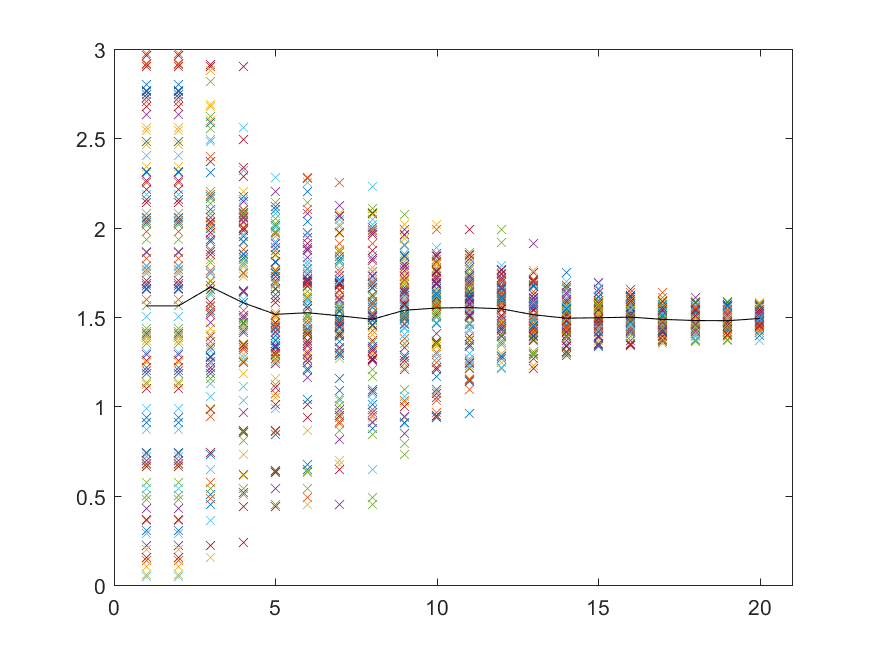
\includegraphics[scale=0.35]{figure/graphs1run/aggressC}}
    \subfloat[][Choleric - II run] {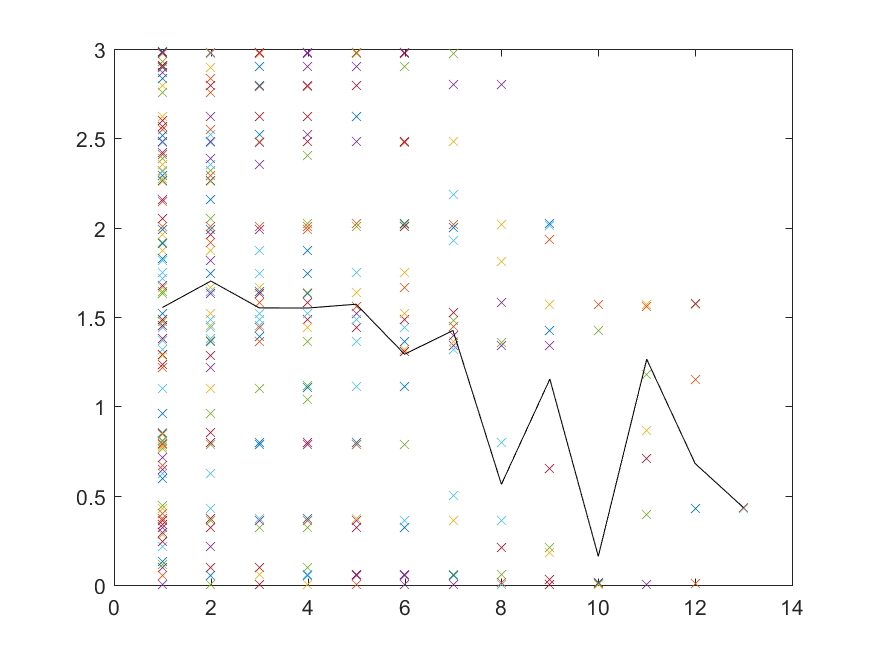
\includegraphics[scale=0.35]{figure/graphs2run/aggressC}}
	\subfloat[][Choleric - III run] {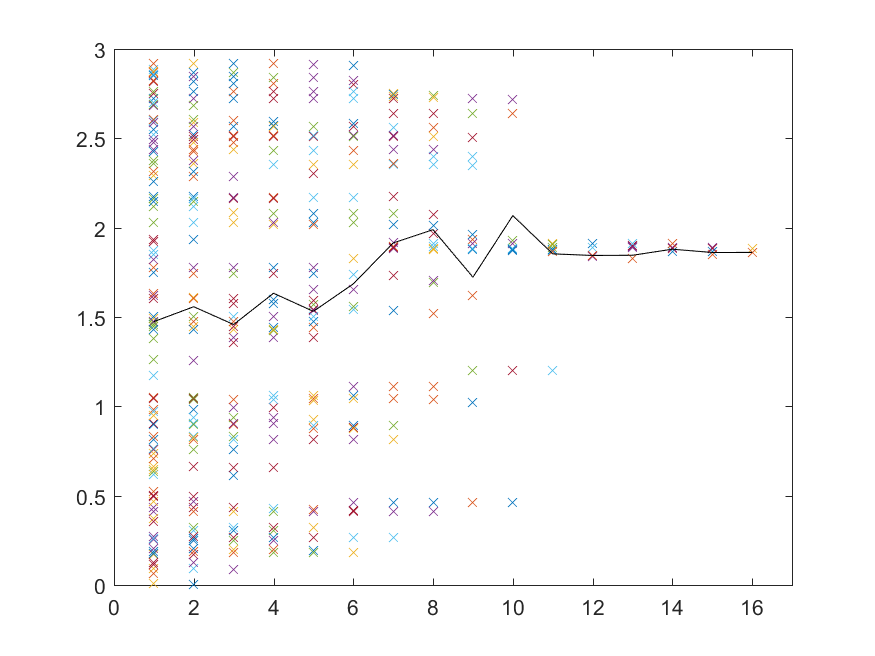
\includegraphics[scale=0.35]{figure/graphs3run/aggressC}}
    \qquad
    \subfloat[][Melancholic - I run]{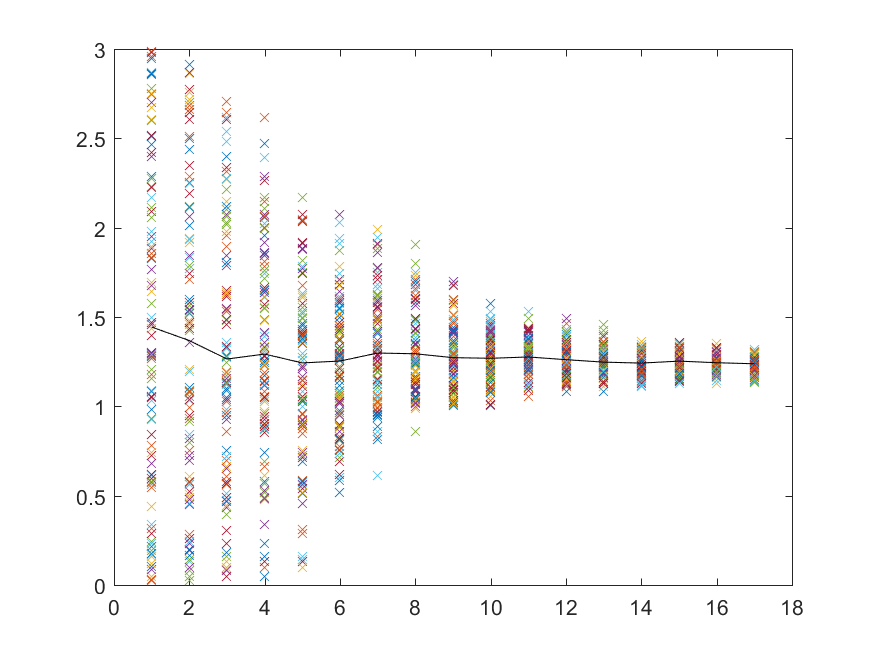
\includegraphics[scale=0.35]{figure/graphs1run/aggressM}}
    \subfloat[][Melancholic - II run]{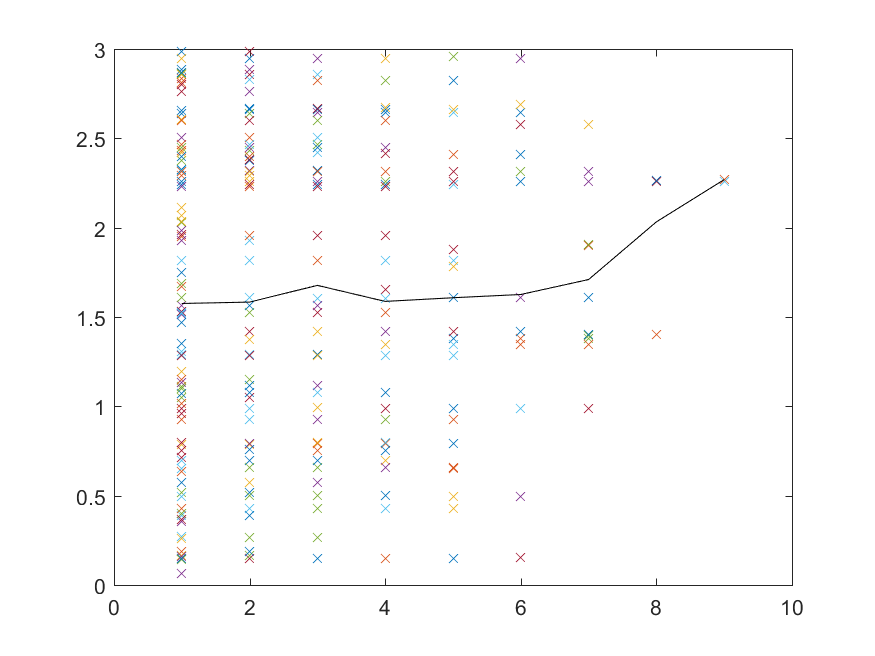
\includegraphics[scale=0.35]{figure/graphs2run/aggressM}}
    \subfloat[][Melancholic - III run]{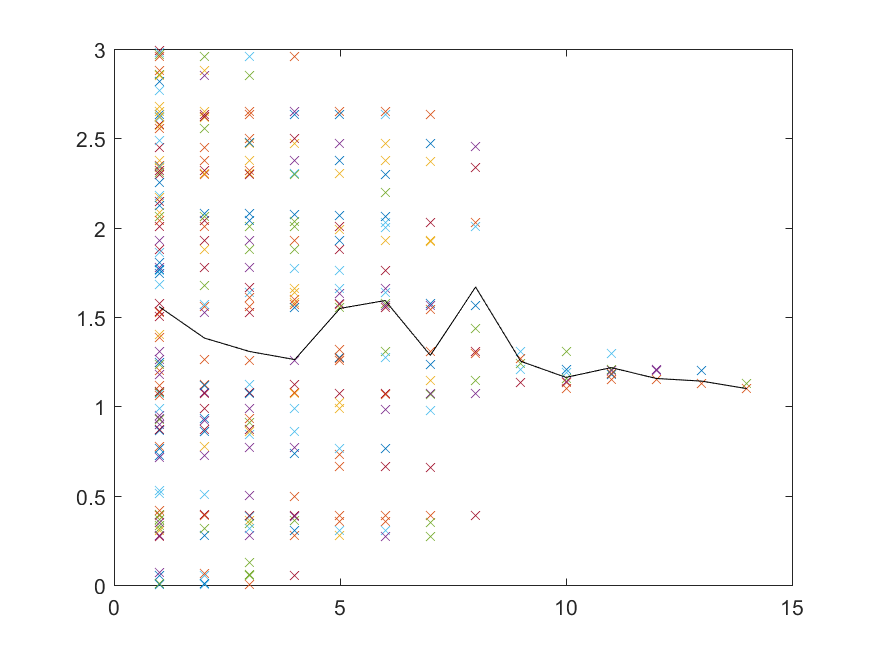
\includegraphics[scale=0.35]{figure/graphs3run/aggressM}}
    \qquad
    \subfloat[][Sanguine - I run]{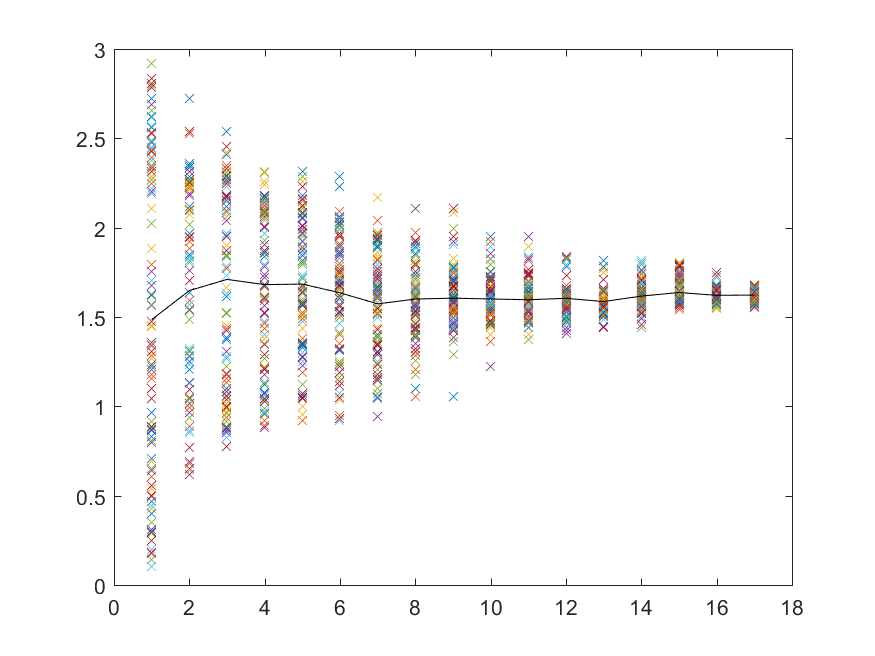
\includegraphics[scale=0.35]{figure/graphs1run/aggressS}}
	\subfloat[][Sanguine - II run]{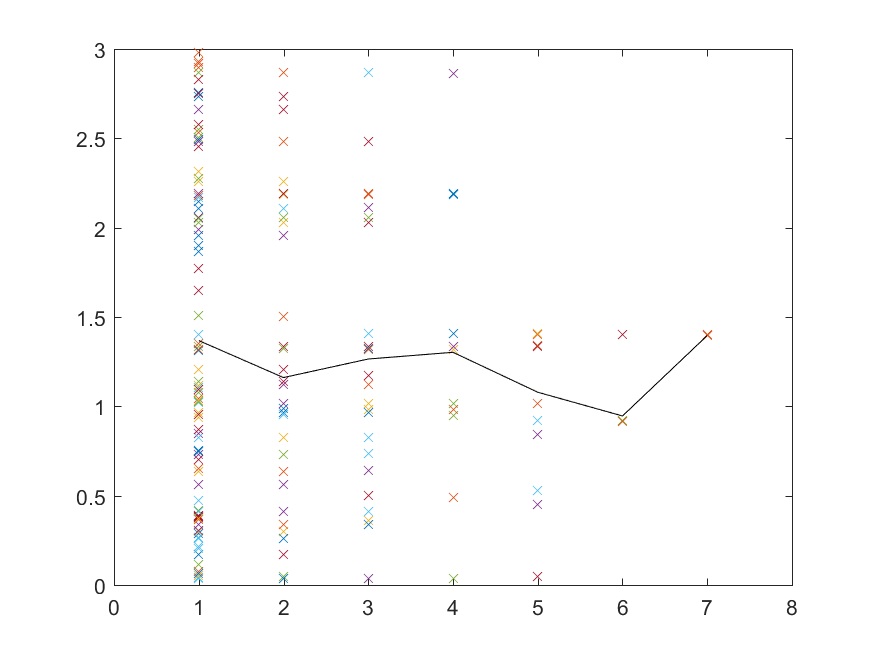
\includegraphics[scale=0.35]{figure/graphs2run/aggressS}}
	\subfloat[][Sanguine - III run]{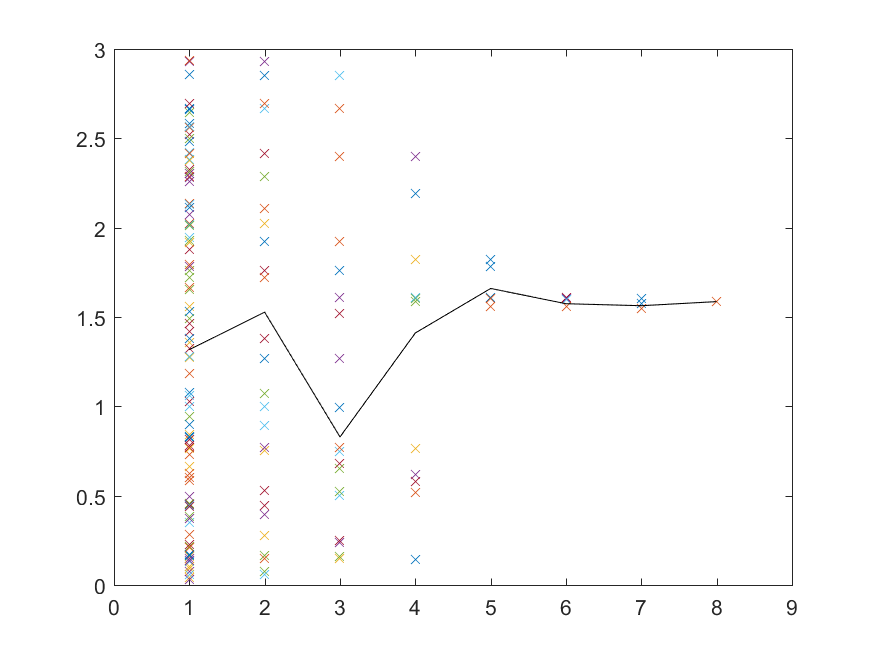
\includegraphics[scale=0.35]{figure/graphs3run/aggressS}}
	\qquad
    \subfloat[][Phlegmatic - I run]{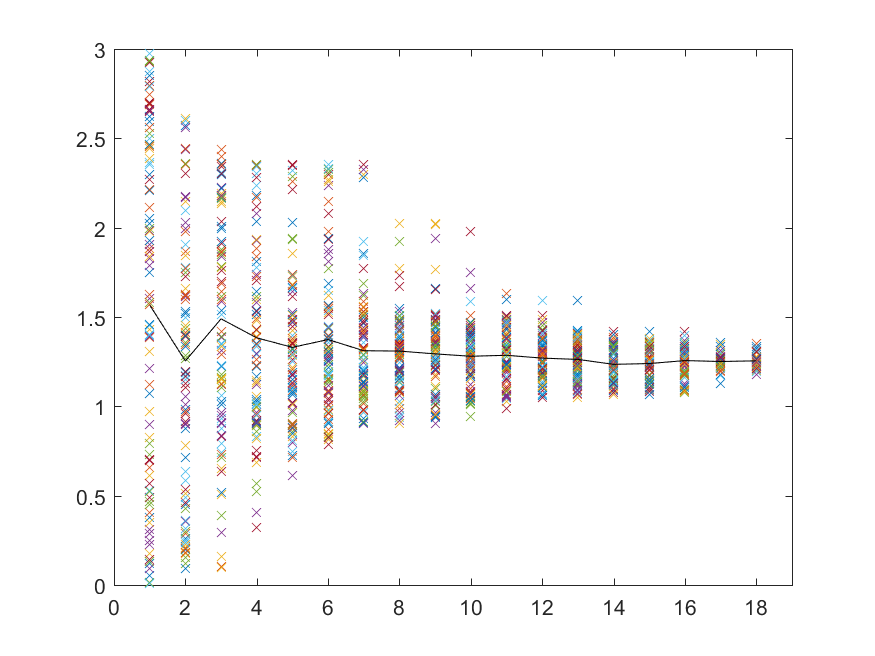
\includegraphics[scale=0.35]{figure/graphs1run/aggressP}}
    \subfloat[][Phlegmatic - II run]{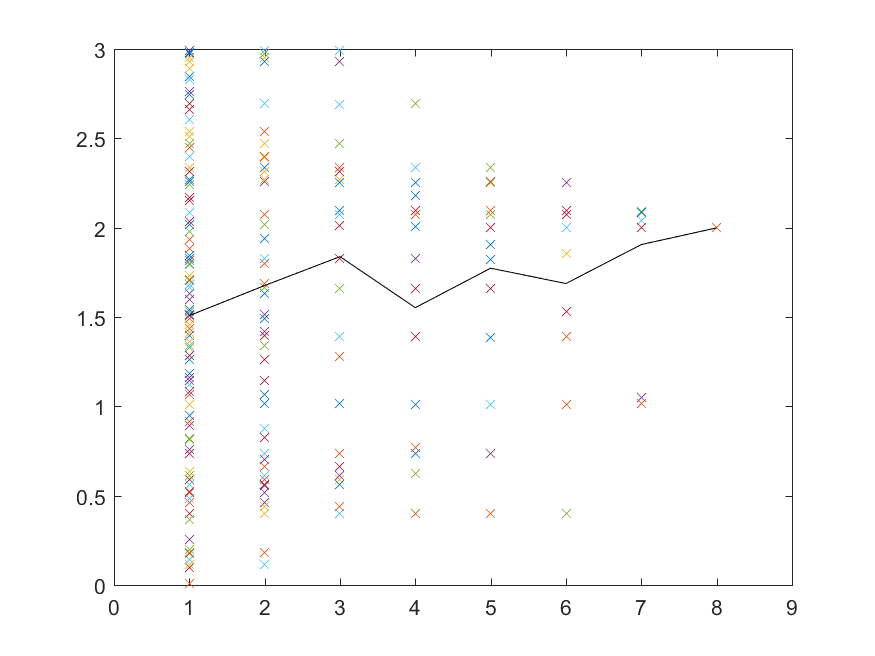
\includegraphics[scale=0.35]{figure/graphs2run/aggressP}}
    \subfloat[][Phlegmatic - III run]{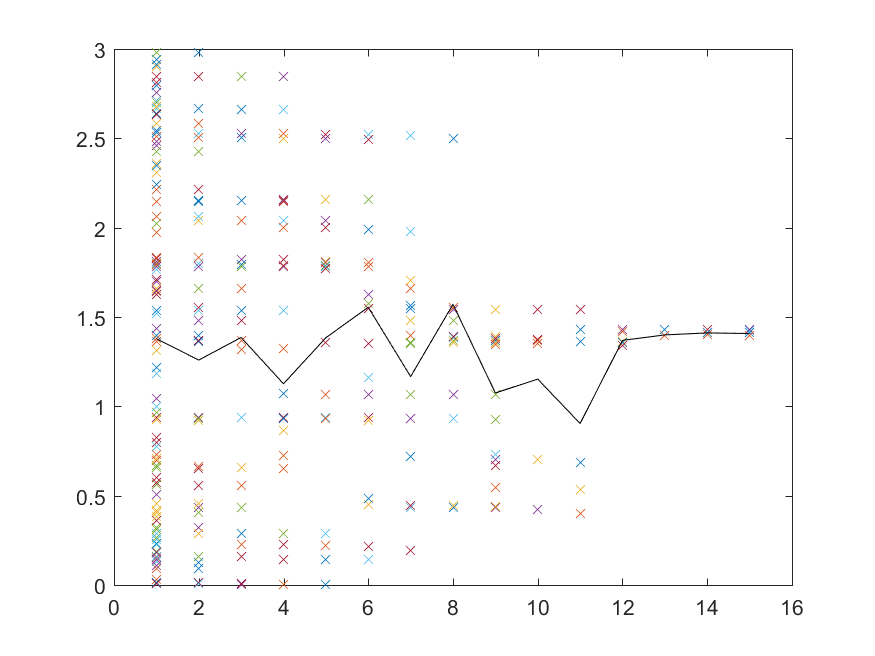
\includegraphics[scale=0.35]{figure/graphs3run/aggressP}}
  \captionsetup{justification=centering}
    \caption{Aggressiveness gene.}
    \label{fig:aggressiveness}
\end{figure}
\vfill
\hspace{0pt}
\pagebreak
\begin{figure}[H]
\centering
    \subfloat[][Choleric - I run] {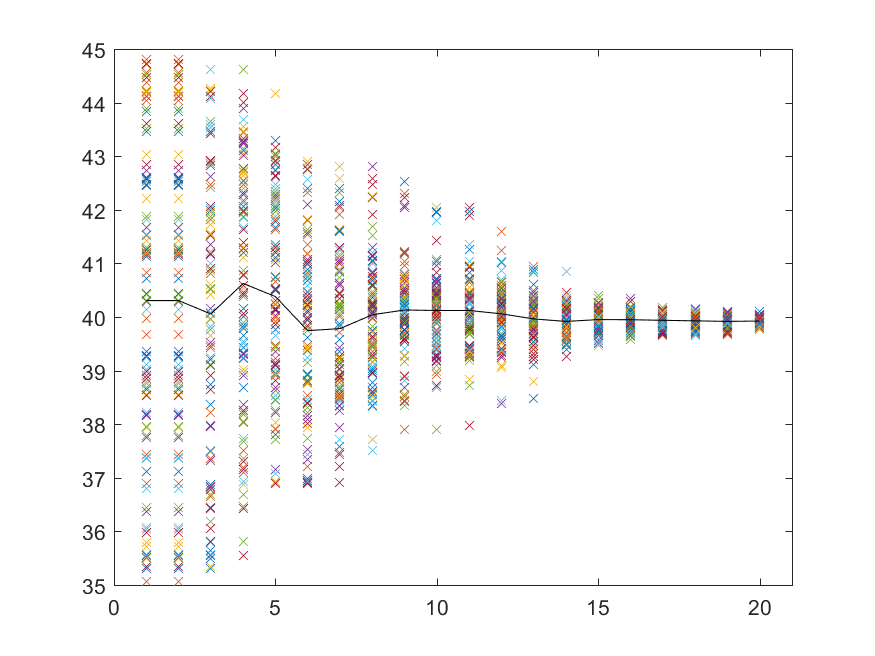
\includegraphics[scale=0.35]{figure/graphs1run/chargedefC}}
    \subfloat[][Choleric - II run] {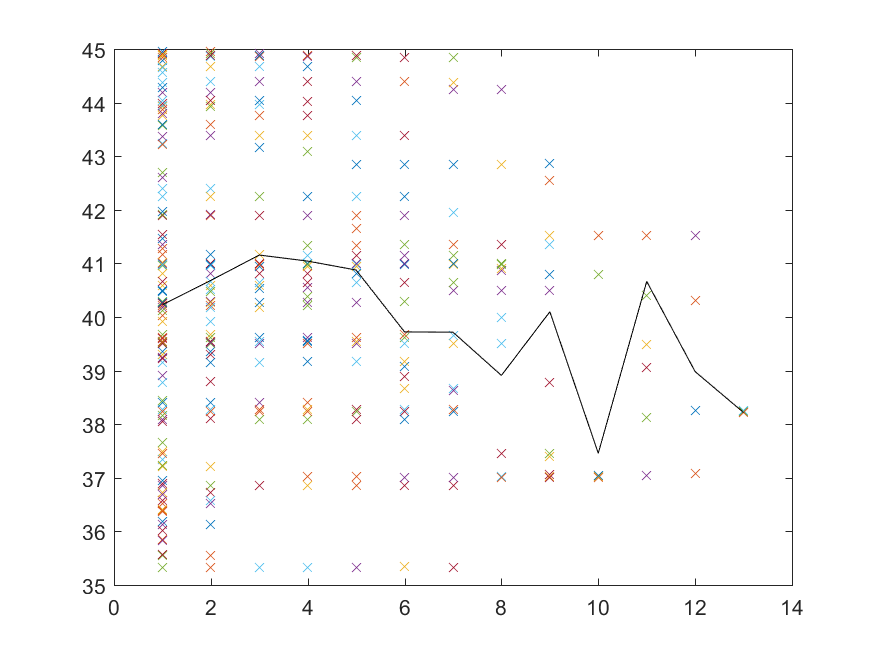
\includegraphics[scale=0.35]{figure/graphs2run/chargedefC}}
	\subfloat[][Choleric - III run] {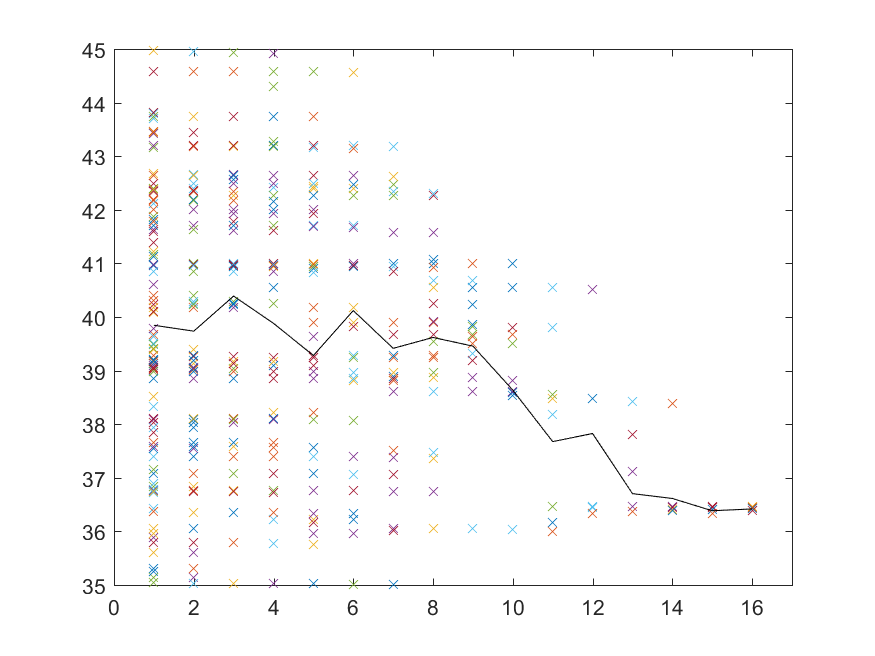
\includegraphics[scale=0.35]{figure/graphs3run/chargedefC}}
    \qquad
    \subfloat[][Melancholic - I run]{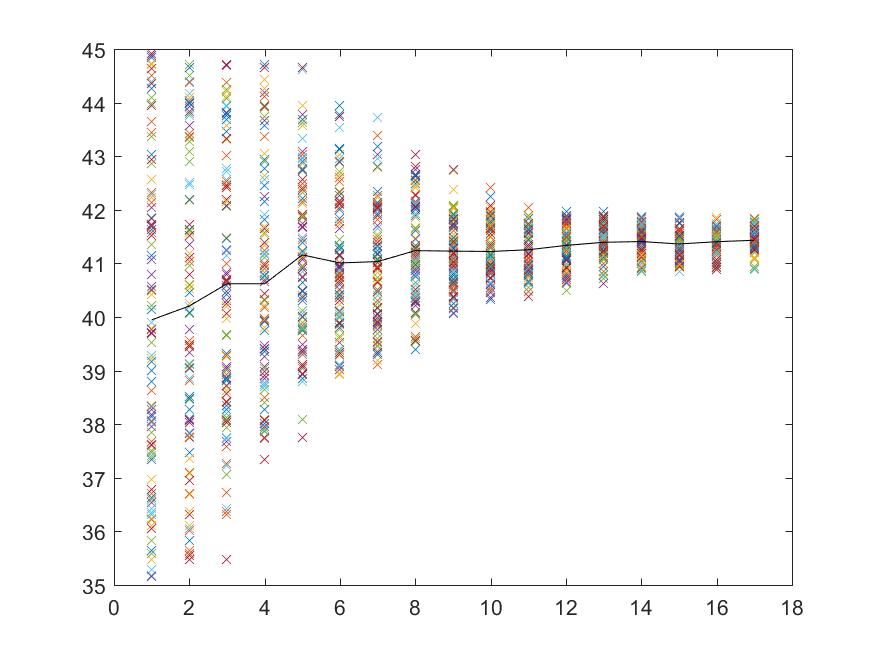
\includegraphics[scale=0.35]{figure/graphs1run/chargedefM}}
    \subfloat[][Melancholic - II run]{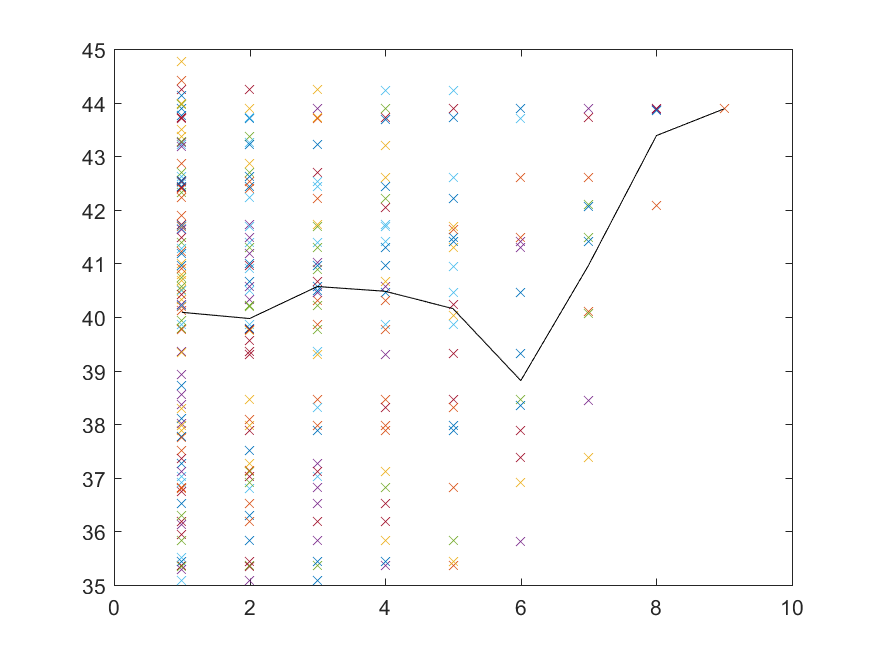
\includegraphics[scale=0.35]{figure/graphs2run/chargedefM}}
    \subfloat[][Melancholic - III run]{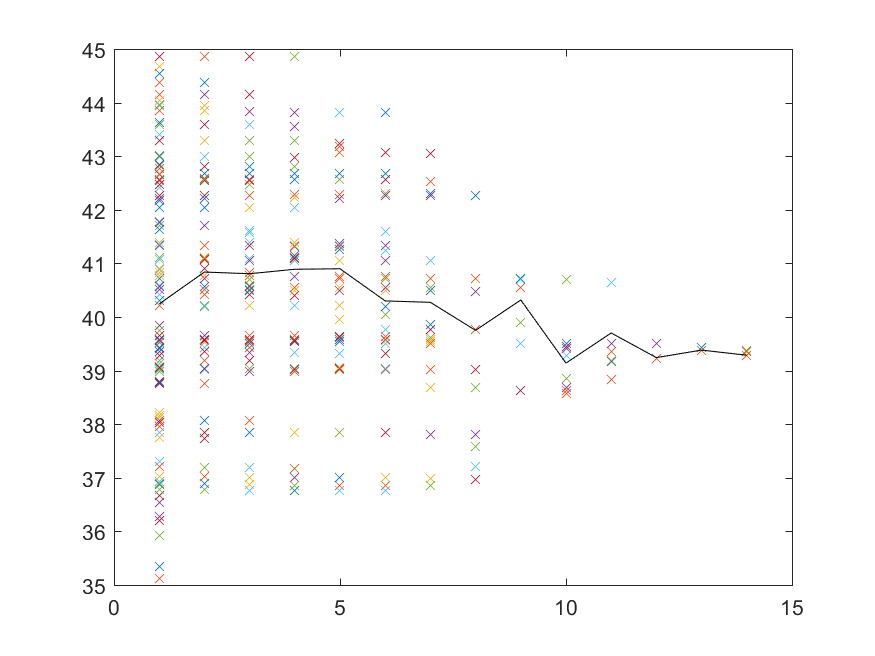
\includegraphics[scale=0.35]{figure/graphs3run/chargedefM}}
    \qquad
    \subfloat[][Sanguine - I run]{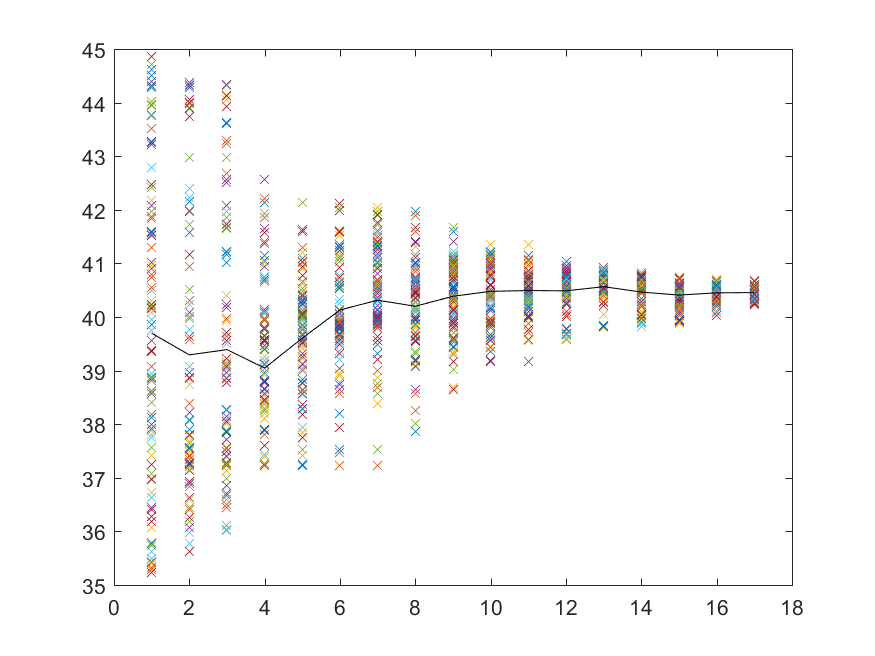
\includegraphics[scale=0.35]{figure/graphs1run/chargedefS}}
	\subfloat[][Sanguine - II run]{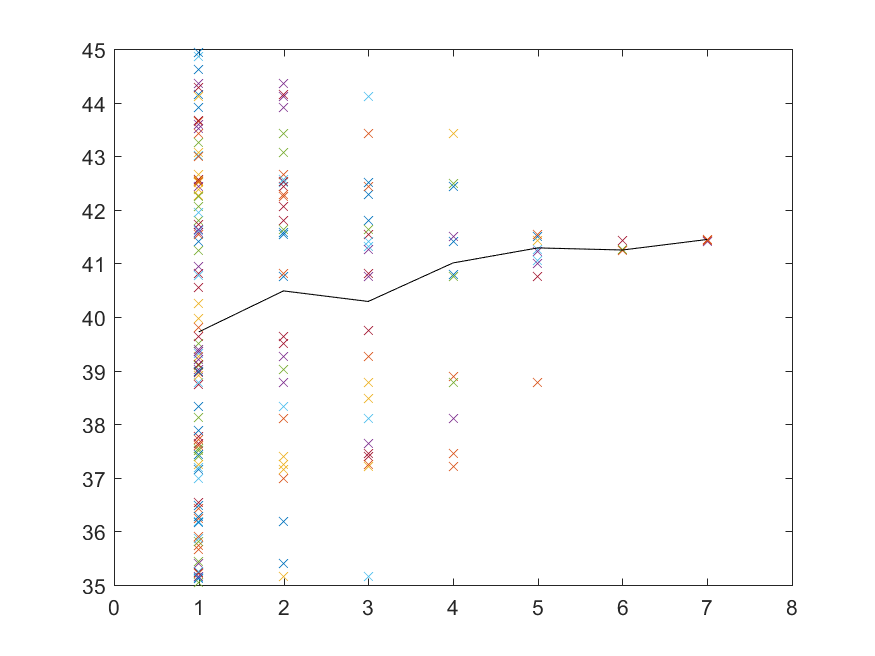
\includegraphics[scale=0.35]{figure/graphs2run/chargedefS}}
	\subfloat[][Sanguine - III run]{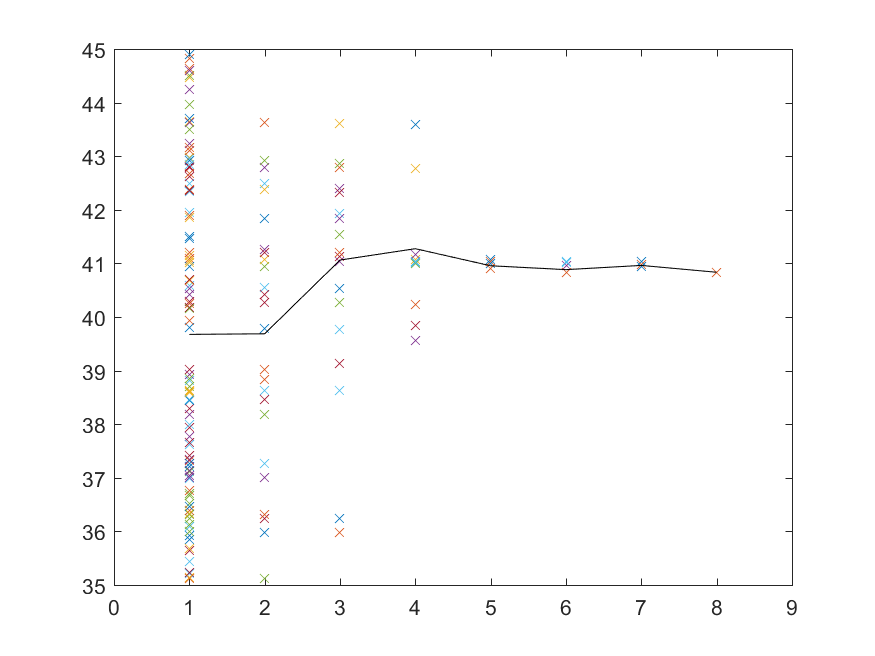
\includegraphics[scale=0.35]{figure/graphs3run/chargedefS}}
	\qquad
    \subfloat[][Phlegmatic - I run]{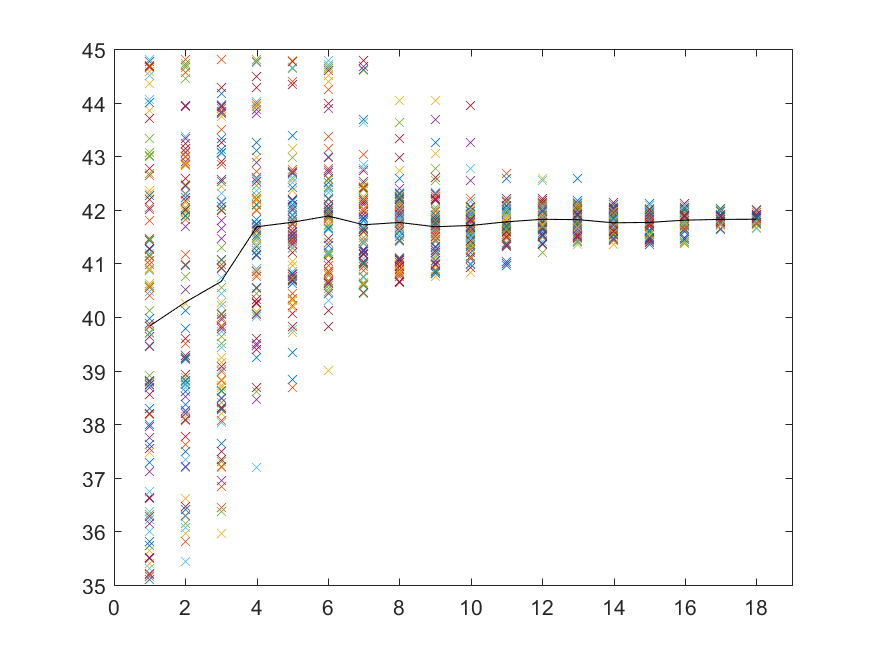
\includegraphics[scale=0.35]{figure/graphs1run/chargedefP}}
    \subfloat[][Phlegmatic - II run]{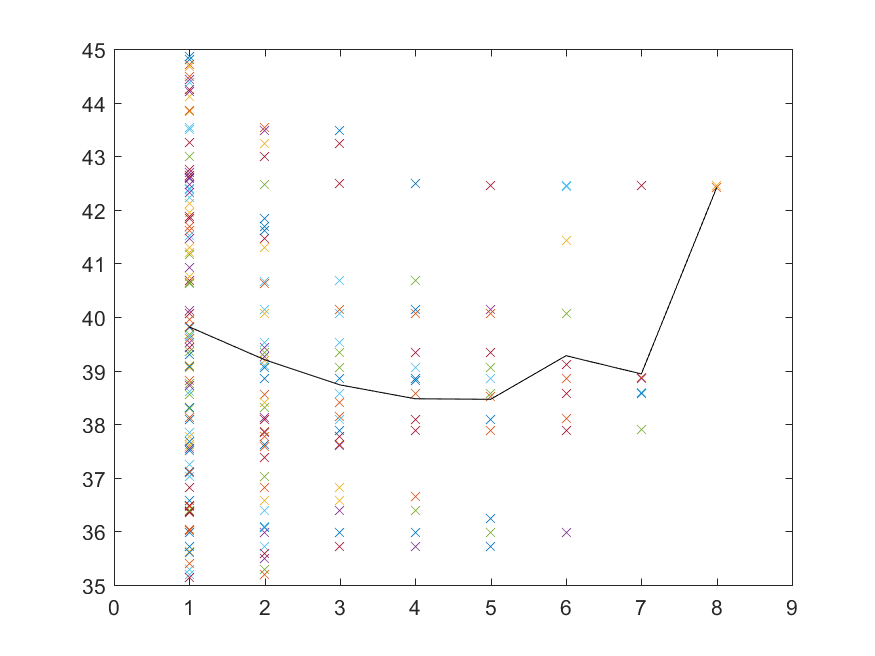
\includegraphics[scale=0.35]{figure/graphs2run/chargedefP}}
    \subfloat[][Phlegmatic - III run]{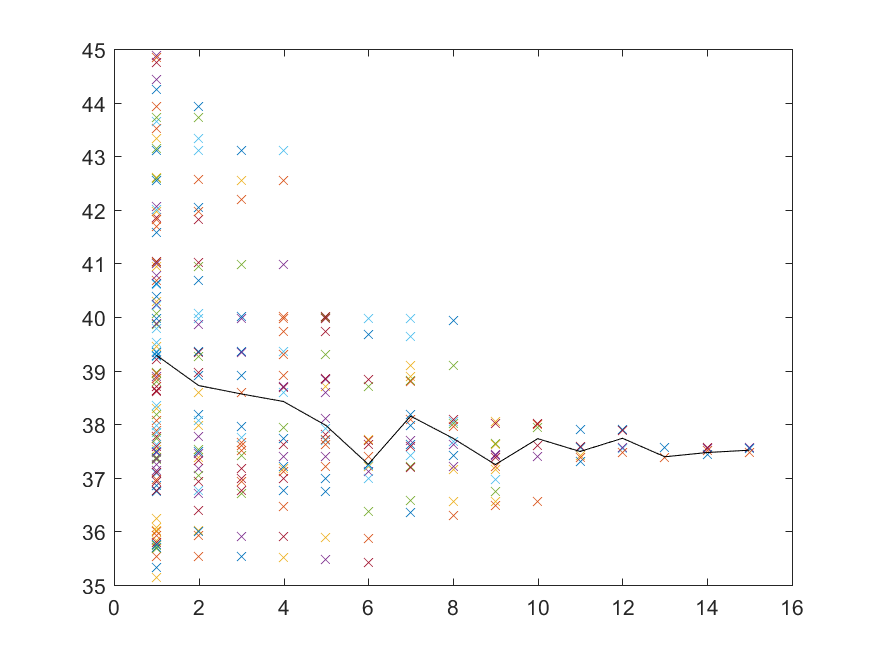
\includegraphics[scale=0.35]{figure/graphs3run/chargedefP}}
  \captionsetup{justification=centering}
    \caption{Charge Default gene.}
    \label{fig:chargedef}
\end{figure}
\begin{figure}[H]
\centering
    \subfloat[][Choleric - I run] {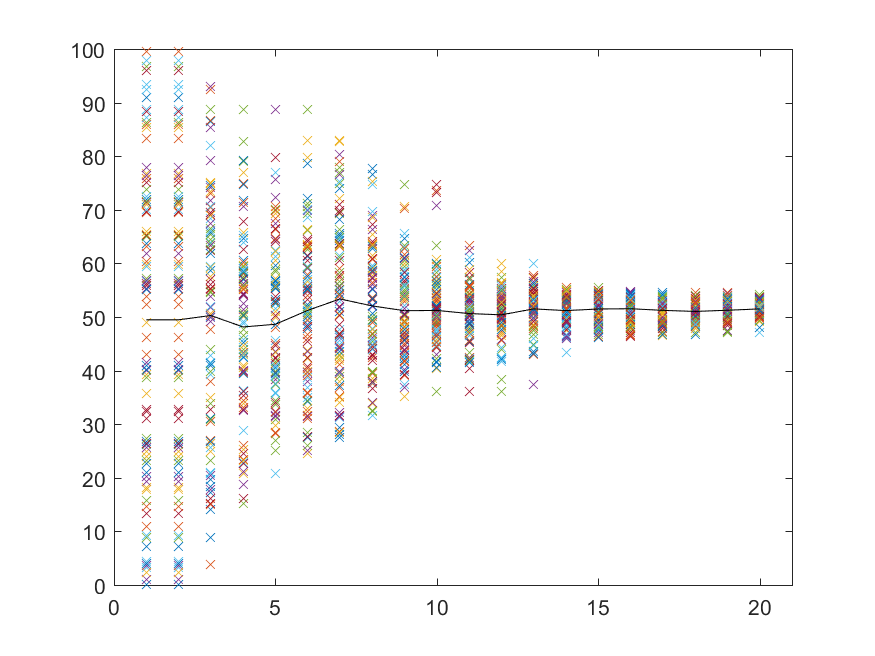
\includegraphics[scale=0.35]{figure/graphs1run/chargedepthC}}
    \subfloat[][Choleric - II run] {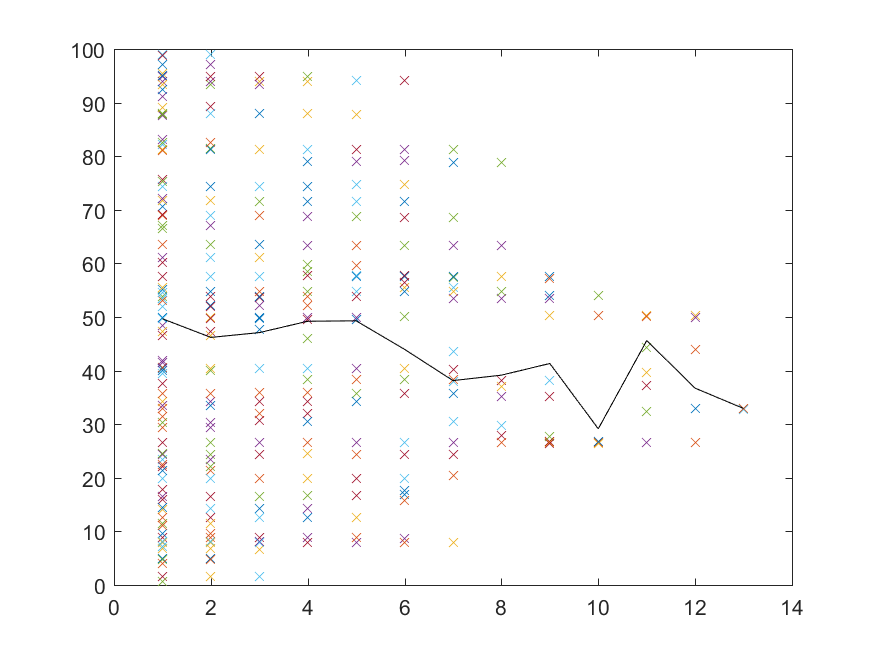
\includegraphics[scale=0.35]{figure/graphs2run/chargedepthC}}
	\subfloat[][Choleric - III run] {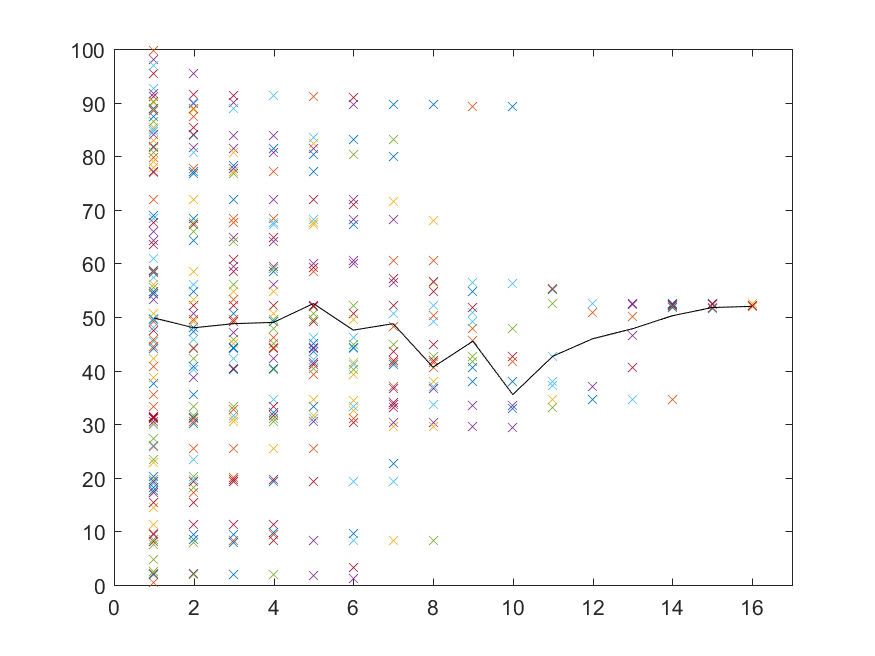
\includegraphics[scale=0.35]{figure/graphs3run/chargedepthC}}
    \qquad
    \subfloat[][Melancholic - I run]{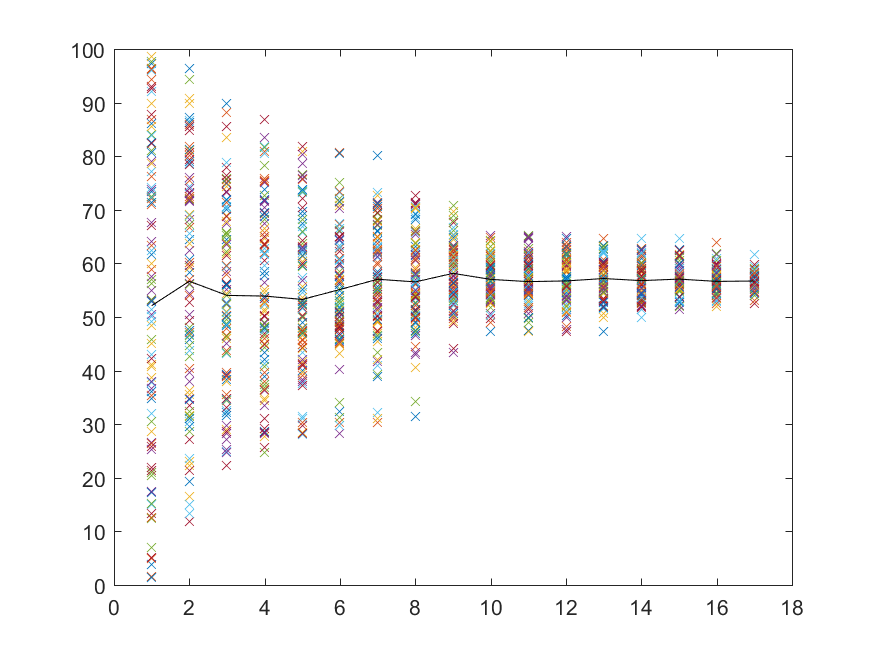
\includegraphics[scale=0.35]{figure/graphs1run/chargedepthM}}
    \subfloat[][Melancholic - II run]{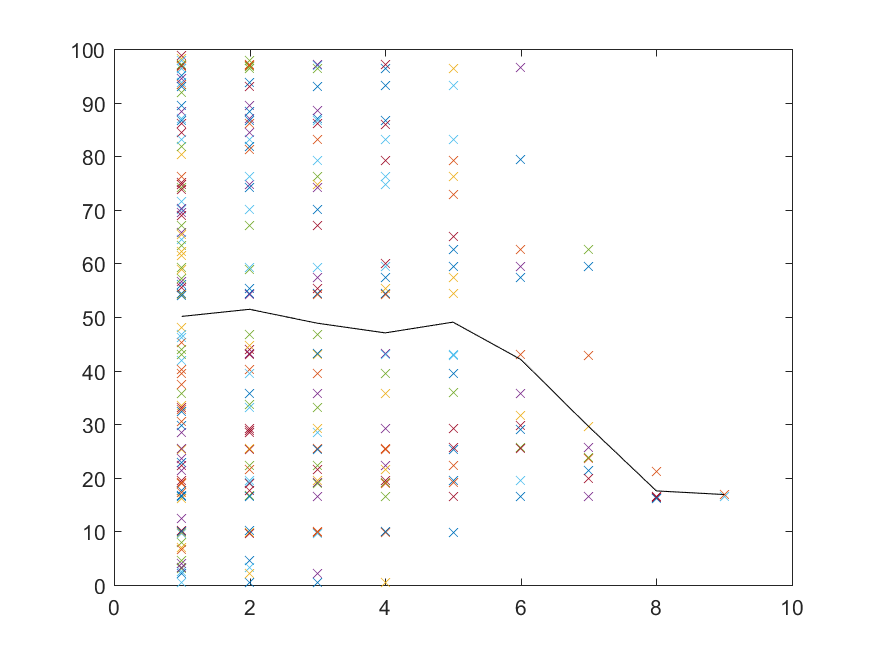
\includegraphics[scale=0.35]{figure/graphs2run/chargedepthM}}
    \subfloat[][Melancholic - III run]{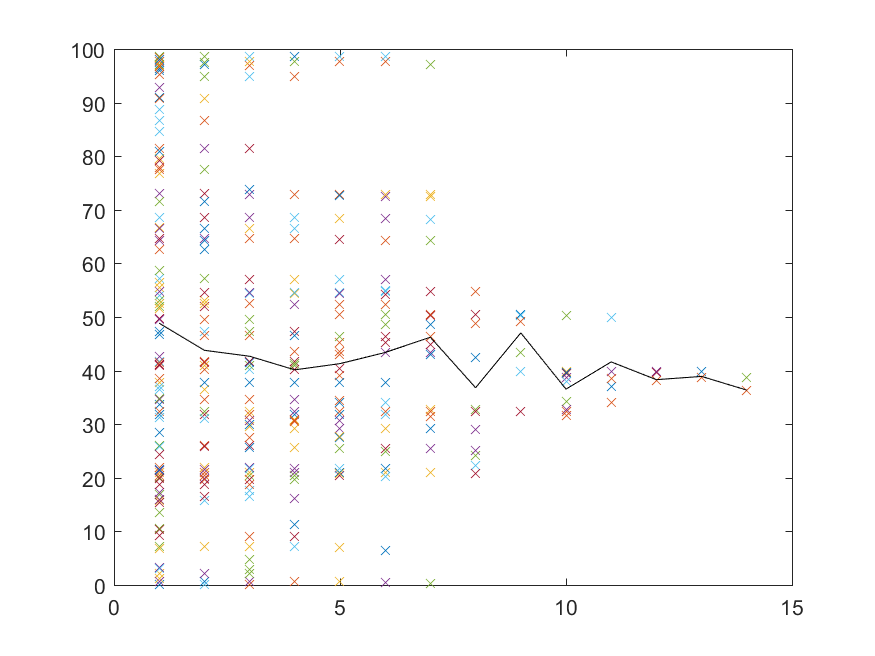
\includegraphics[scale=0.35]{figure/graphs3run/chargedepthM}}
    \qquad
    \subfloat[][Sanguine - I run]{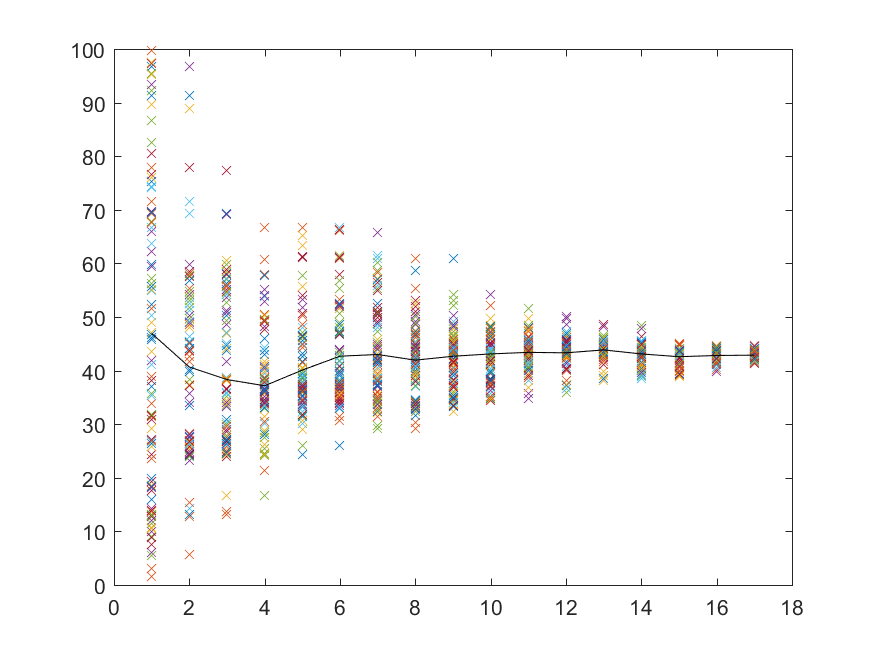
\includegraphics[scale=0.35]{figure/graphs1run/chargedepthS}}
	\subfloat[][Sanguine - II run]{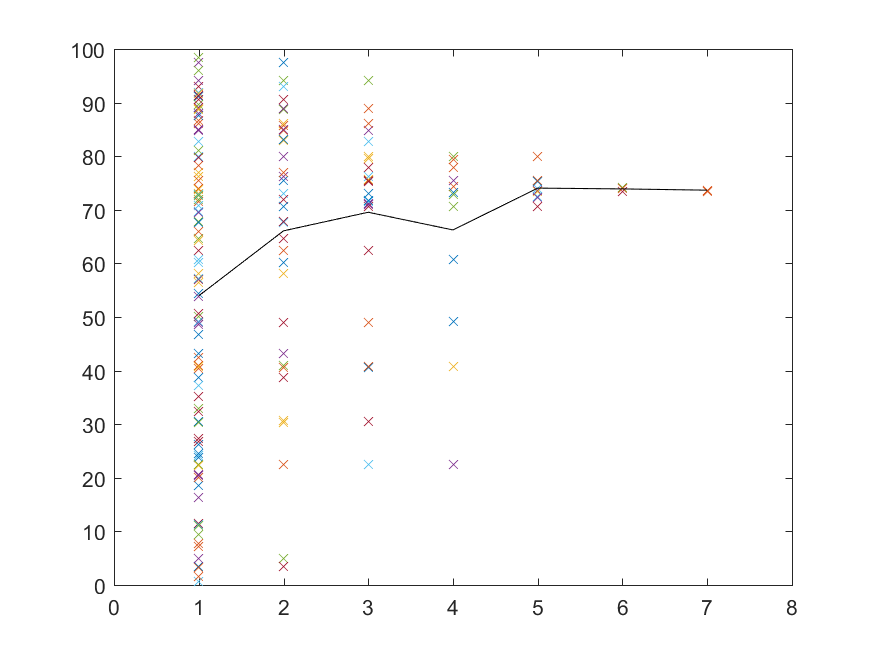
\includegraphics[scale=0.35]{figure/graphs2run/chargedepthS}}
	\subfloat[][Sanguine - III run]{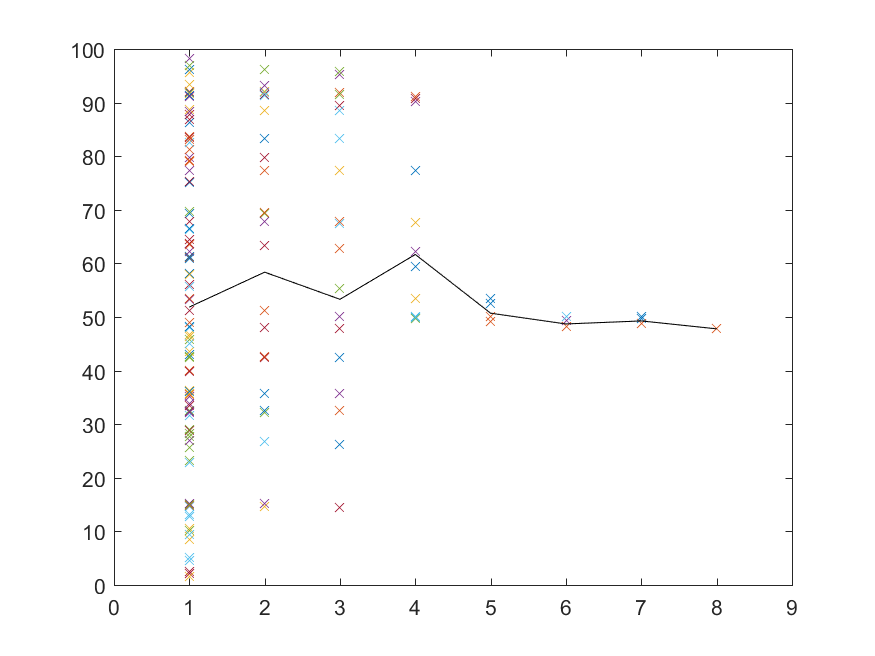
\includegraphics[scale=0.35]{figure/graphs3run/chargedepthS}}
	\qquad
    \subfloat[][Phlegmatic - I run]{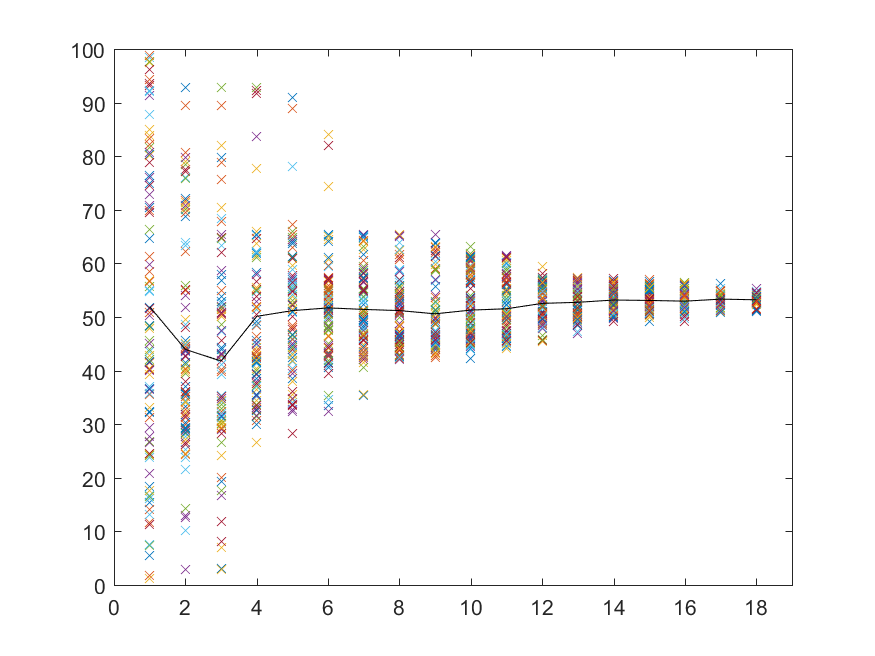
\includegraphics[scale=0.35]{figure/graphs1run/chargedepthP}}
    \subfloat[][Phlegmatic - II run]{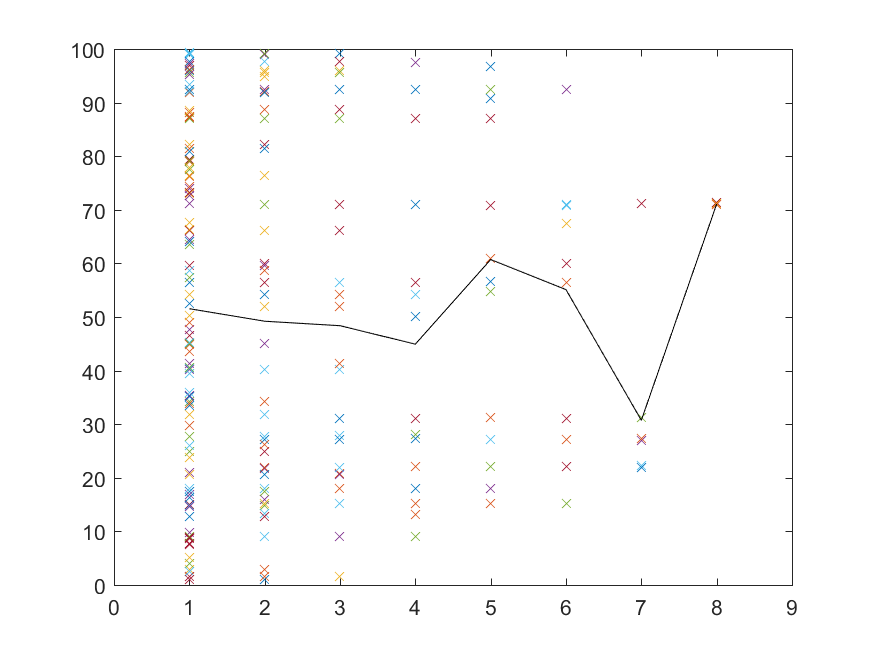
\includegraphics[scale=0.35]{figure/graphs2run/chargedepthP}}
    \subfloat[][Phlegmatic - III run]{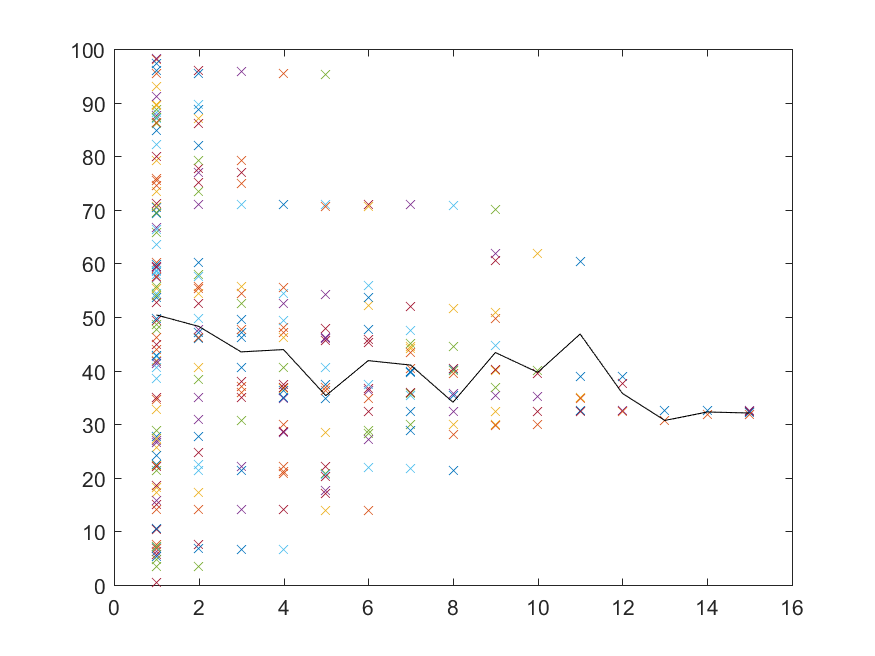
\includegraphics[scale=0.35]{figure/graphs3run/chargedepthP}}
  \captionsetup{justification=centering}
    \caption{Charge Depth gene.}
    \label{fig:chargedepth}
\end{figure}
\begin{figure}[H]
\centering
    \subfloat[][Choleric - I run] {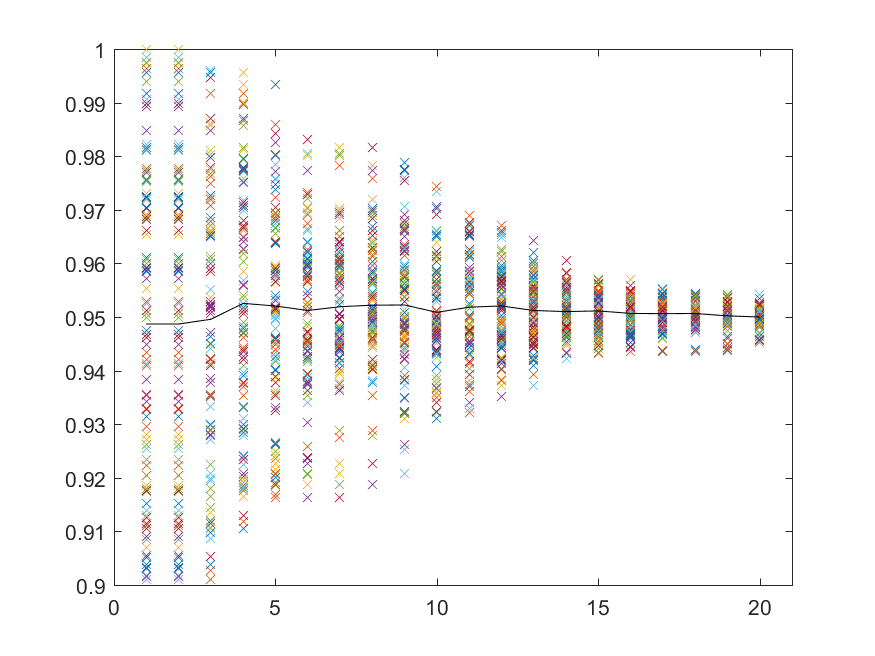
\includegraphics[scale=0.35]{figure/graphs1run/chargediscountC}}
    \subfloat[][Choleric - II run] {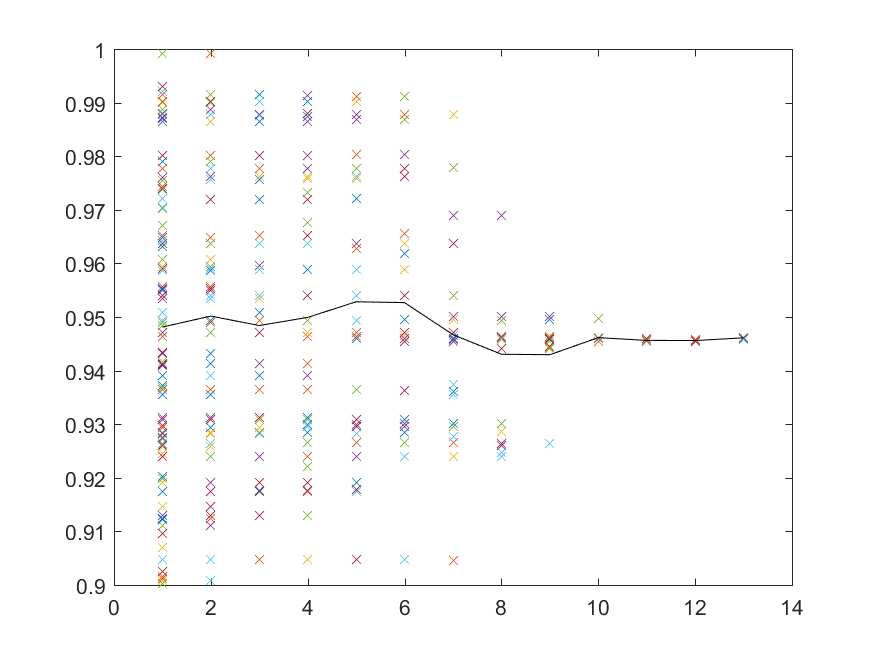
\includegraphics[scale=0.35]{figure/graphs2run/chargediscountC}}
	\subfloat[][Choleric - III run] {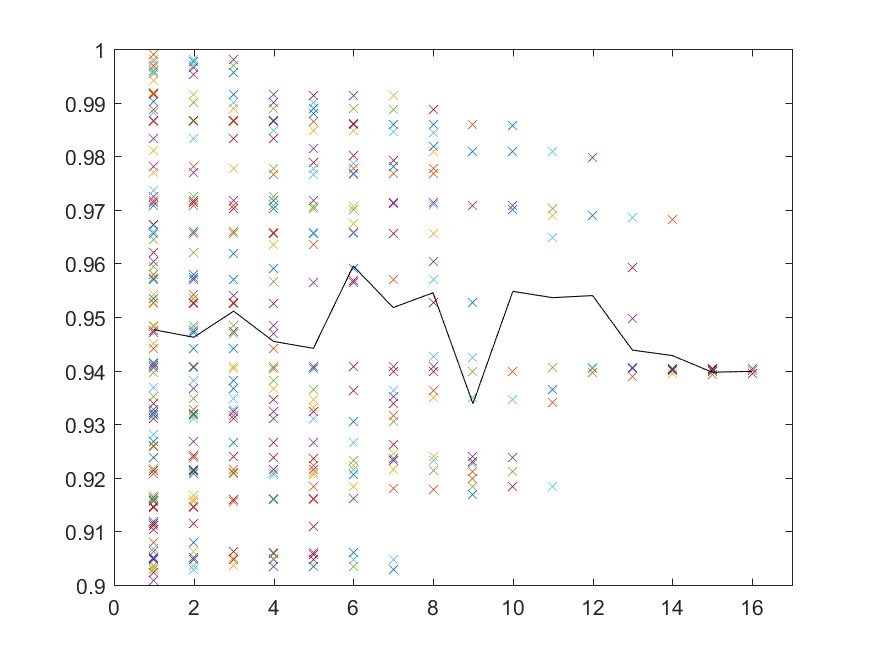
\includegraphics[scale=0.35]{figure/graphs3run/chargediscountC}}
    \qquad
    \subfloat[][Melancholic - I run]{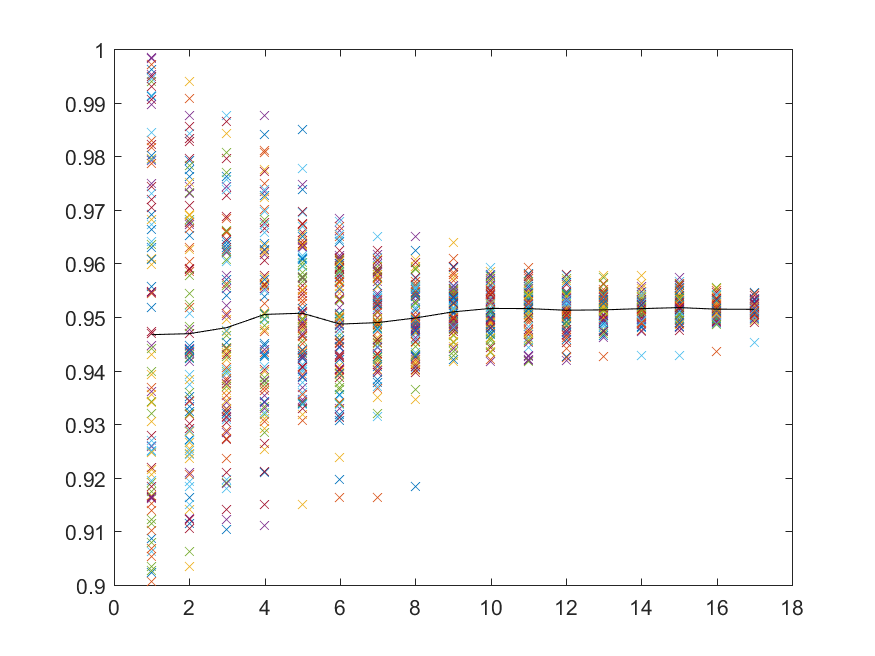
\includegraphics[scale=0.35]{figure/graphs1run/chargediscountM}}
    \subfloat[][Melancholic - II run]{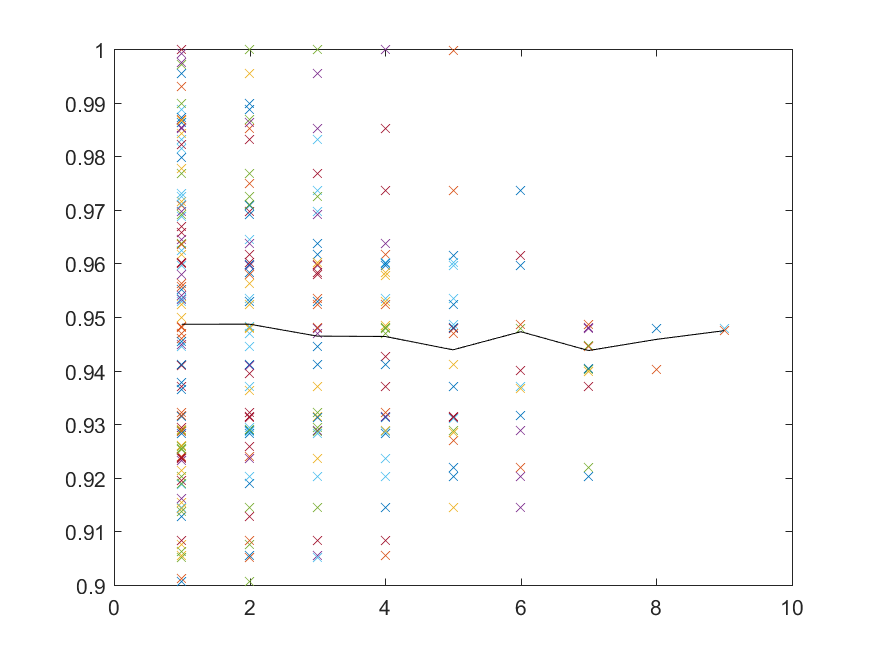
\includegraphics[scale=0.35]{figure/graphs2run/chargediscountM}}
    \subfloat[][Melancholic - III run]{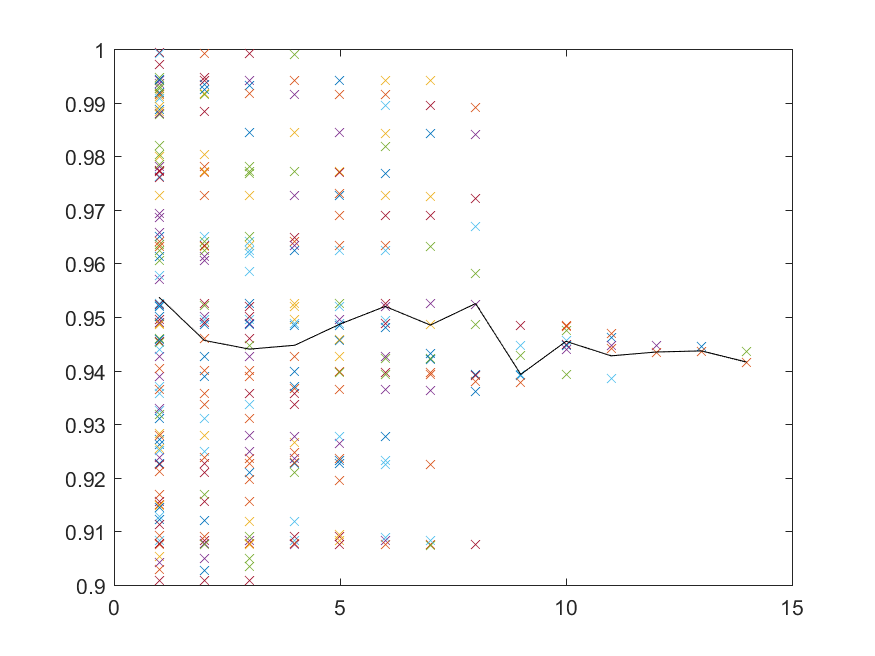
\includegraphics[scale=0.35]{figure/graphs3run/chargediscountM}}
    \qquad
    \subfloat[][Sanguine - I run]{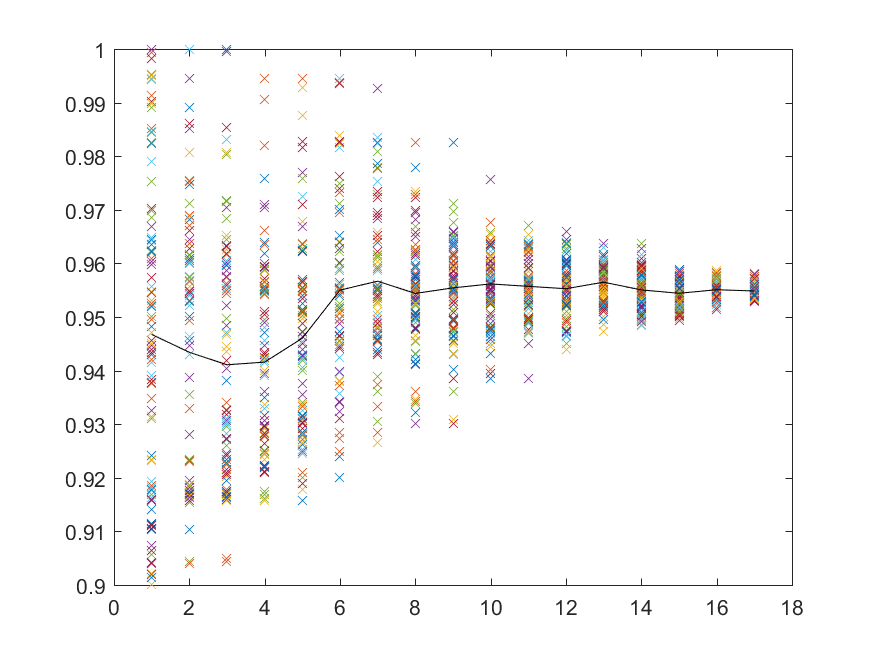
\includegraphics[scale=0.35]{figure/graphs1run/chargediscountS}}
	\subfloat[][Sanguine - II run]{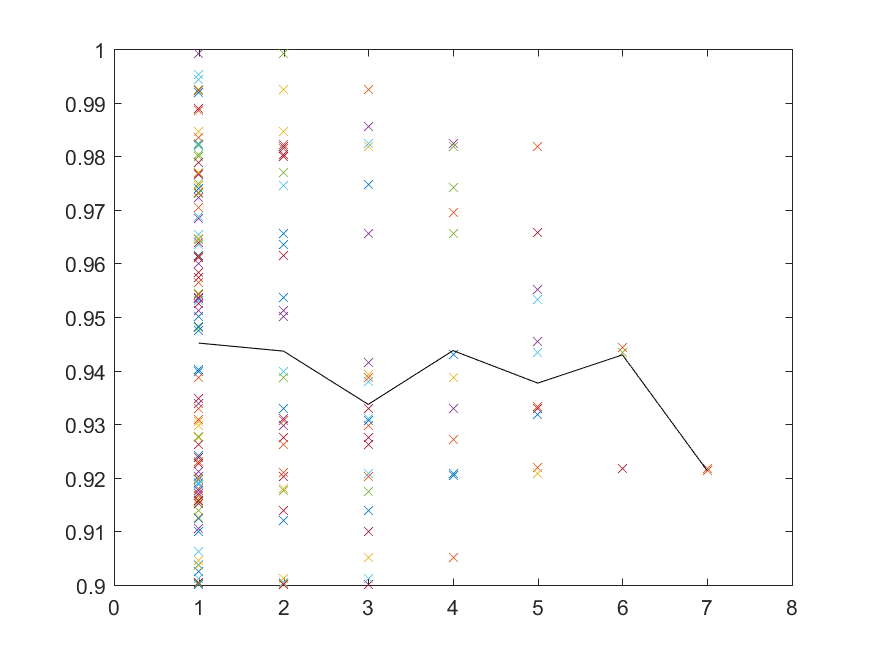
\includegraphics[scale=0.35]{figure/graphs2run/chargediscountS}}
	\subfloat[][Sanguine - III run]{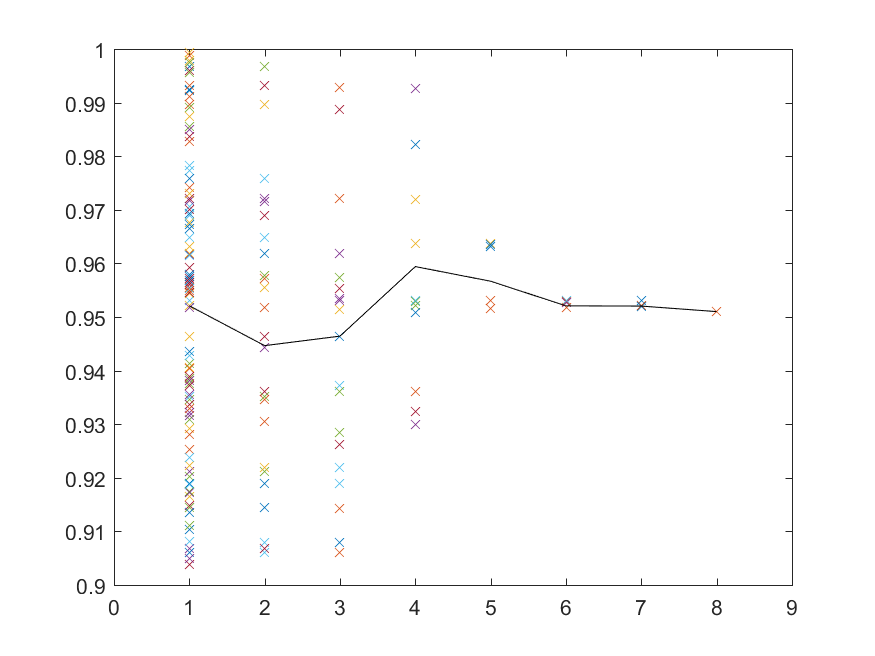
\includegraphics[scale=0.35]{figure/graphs3run/chargediscountS}}
	\qquad
    \subfloat[][Phlegmatic - I run]{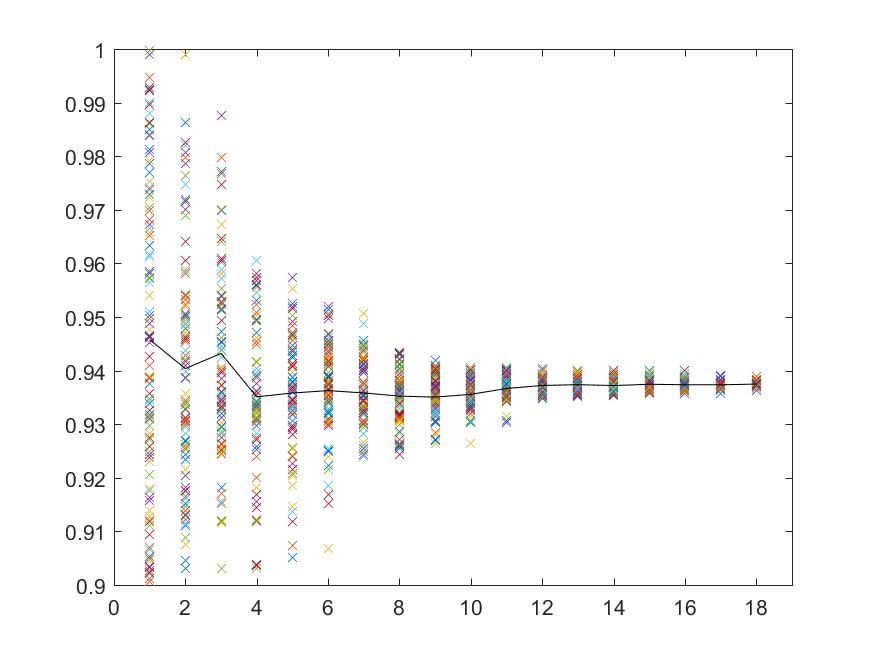
\includegraphics[scale=0.35]{figure/graphs1run/chargediscountP}}
    \subfloat[][Phlegmatic - II run]{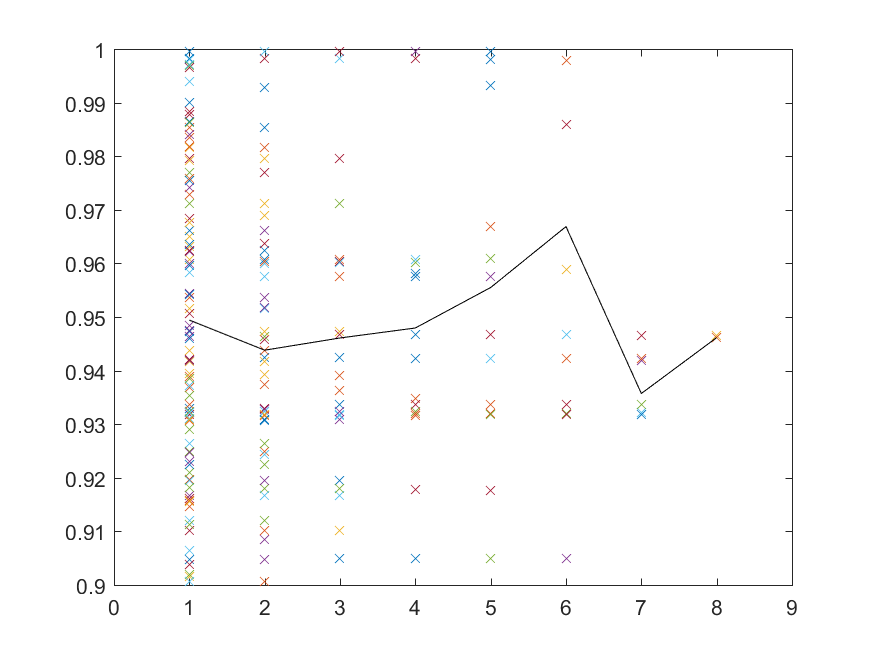
\includegraphics[scale=0.35]{figure/graphs2run/chargediscountP}}
    \subfloat[][Phlegmatic - III run]{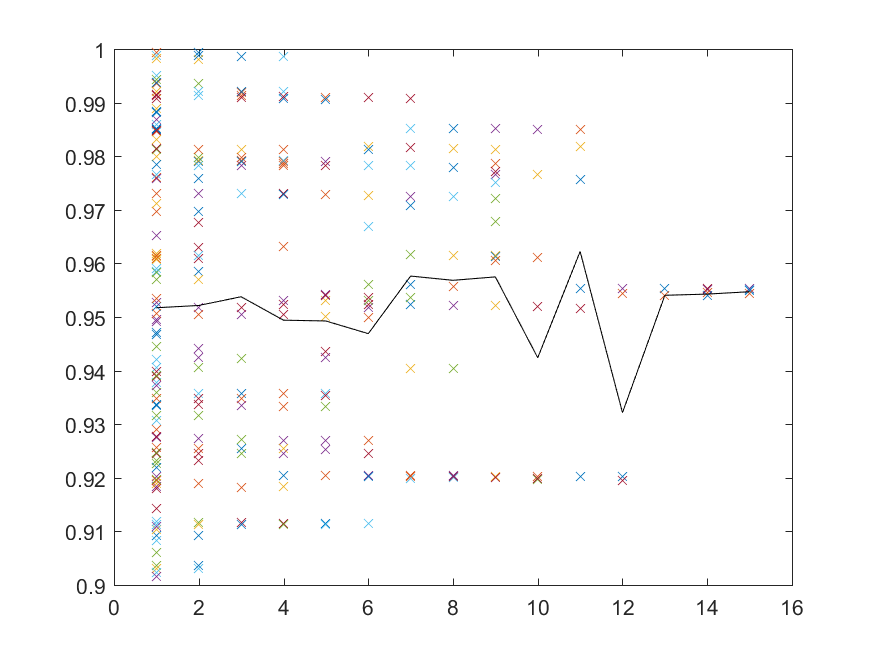
\includegraphics[scale=0.35]{figure/graphs3run/chargediscountP}}
  \captionsetup{justification=centering}
    \caption{Charge Discount gene.}
    \label{fig:chargediscount}
\end{figure}
\begin{figure}[H]
\centering
    \subfloat[][Choleric - I run] {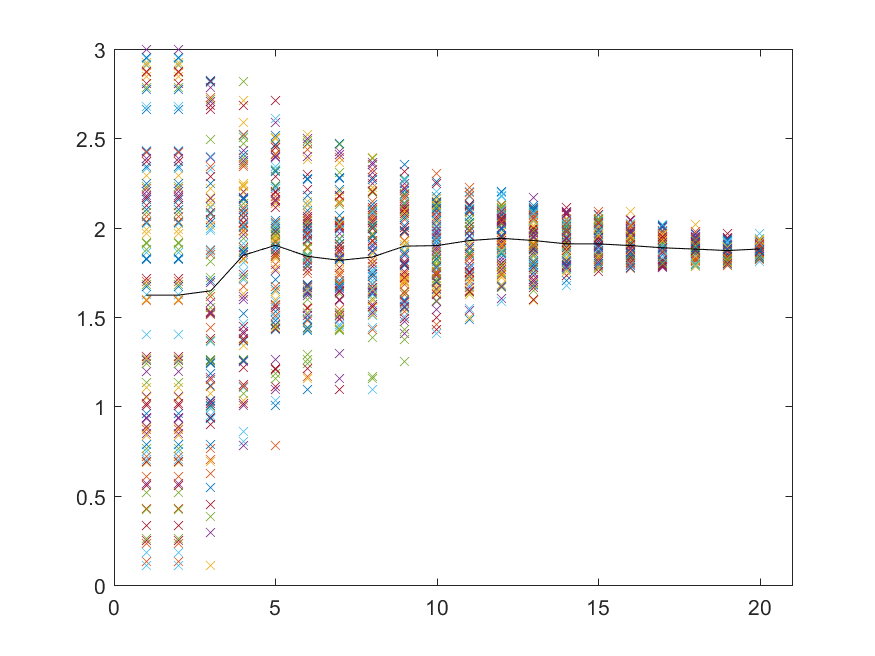
\includegraphics[scale=0.35]{figure/graphs1run/defensivC}}
    \subfloat[][Choleric - II run] {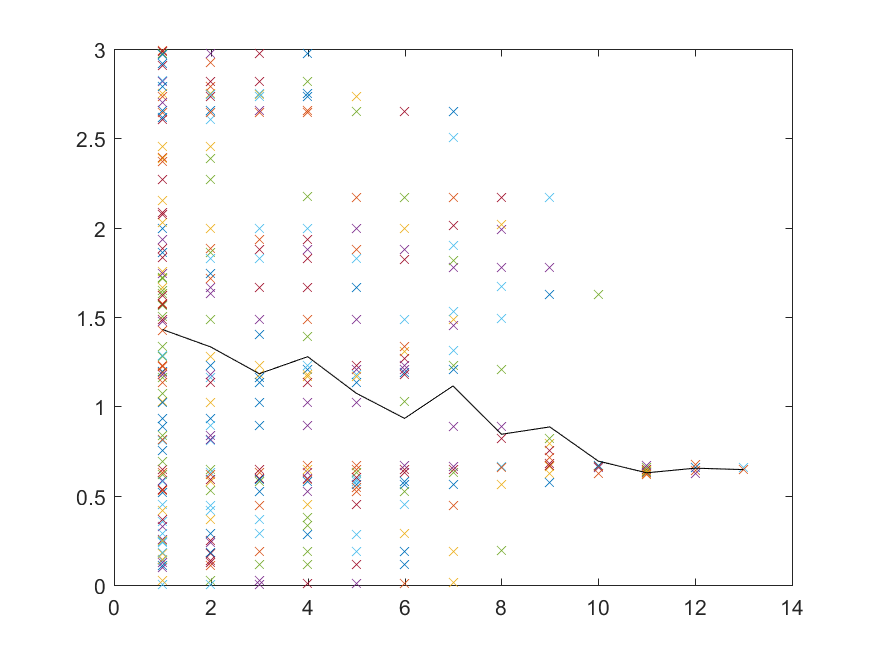
\includegraphics[scale=0.35]{figure/graphs2run/defensivC}}
	\subfloat[][Choleric - III run] {\includegraphics[scale=0.35]{figure/graphs3run/defensivC}}
    \qquad
    \subfloat[][Melancholic - I run]{\includegraphics[scale=0.35]{figure/graphs1run/defensivM}}
    \subfloat[][Melancholic - II run]{\includegraphics[scale=0.35]{figure/graphs2run/defensivM}}
    \subfloat[][Melancholic - III run]{\includegraphics[scale=0.35]{figure/graphs3run/defensivM}}
    \qquad
    \subfloat[][Sanguine - I run]{\includegraphics[scale=0.35]{figure/graphs1run/defensivS}}
	\subfloat[][Sanguine - II run]{\includegraphics[scale=0.35]{figure/graphs2run/defensivS}}
	\subfloat[][Sanguine - III run]{\includegraphics[scale=0.35]{figure/graphs3run/defensivS}}
	\qquad
    \subfloat[][Phlegmatic - I run]{\includegraphics[scale=0.35]{figure/graphs1run/defensivP}}
    \subfloat[][Phlegmatic - II run]{\includegraphics[scale=0.35]{figure/graphs2run/defensivP}}
    \subfloat[][Phlegmatic - III run]{\includegraphics[scale=0.35]{figure/graphs3run/defensivP}}
  \captionsetup{justification=centering}
    \caption{Defensiveness gene.}
    \label{fig:defensiveness}
\end{figure}
\begin{figure}[H]
\centering
    \subfloat[][Choleric - I run] {\includegraphics[scale=0.35]{figure/graphs1run/epsilonC}}
    \subfloat[][Choleric - II run] {\includegraphics[scale=0.35]{figure/graphs2run/epsilonC}}
	\subfloat[][Choleric - III run] {\includegraphics[scale=0.35]{figure/graphs3run/epsilonC}}
    \qquad
    \subfloat[][Melancholic - I run]{\includegraphics[scale=0.35]{figure/graphs1run/epsilonM}}
    \subfloat[][Melancholic - II run]{\includegraphics[scale=0.35]{figure/graphs2run/epsilonM}}
    \subfloat[][Melancholic - III run]{\includegraphics[scale=0.35]{figure/graphs3run/epsilonM}}
    \qquad
    \subfloat[][Sanguine - I run]{\includegraphics[scale=0.35]{figure/graphs1run/epsilonS}}
	\subfloat[][Sanguine - II run]{\includegraphics[scale=0.35]{figure/graphs2run/epsilonS}}
	\subfloat[][Sanguine - III run]{\includegraphics[scale=0.35]{figure/graphs3run/epsilonS}}
	\qquad
    \subfloat[][Phlegmatic - I run]{\includegraphics[scale=0.35]{figure/graphs1run/epsilonP}}
    \subfloat[][Phlegmatic - II run]{\includegraphics[scale=0.35]{figure/graphs2run/epsilonP}}
    \subfloat[][Phlegmatic - III run]{\includegraphics[scale=0.35]{figure/graphs3run/epsilonP}}
  \captionsetup{justification=centering}
    \caption{Epsilon gene.}
    \label{fig:epsilon}
\end{figure}
\begin{figure}[H]
\centering
    \subfloat[][Choleric - I run] {\includegraphics[scale=0.35]{figure/graphs1run/explfactC}}
    \subfloat[][Choleric - II run] {\includegraphics[scale=0.35]{figure/graphs2run/explfactC}}
	\subfloat[][Choleric - III run] {\includegraphics[scale=0.35]{figure/graphs3run/explfactC}}
    \qquad
    \subfloat[][Melancholic - I run]{\includegraphics[scale=0.35]{figure/graphs1run/explfactM}}
    \subfloat[][Melancholic - II run]{\includegraphics[scale=0.35]{figure/graphs2run/explfactM}}
    \subfloat[][Melancholic - III run]{\includegraphics[scale=0.35]{figure/graphs3run/explfactM}}
    \qquad
    \subfloat[][Sanguine - I run]{\includegraphics[scale=0.35]{figure/graphs1run/explfactS}}
	\subfloat[][Sanguine - II run]{\includegraphics[scale=0.35]{figure/graphs2run/explfactS}}
	\subfloat[][Sanguine - III run]{\includegraphics[scale=0.35]{figure/graphs3run/explfactS}}
	\qquad
    \subfloat[][Phlegmatic - I run]{\includegraphics[scale=0.35]{figure/graphs1run/explfactP}}
    \subfloat[][Phlegmatic - II run]{\includegraphics[scale=0.35]{figure/graphs2run/explfactP}}
    \subfloat[][Phlegmatic - III run]{\includegraphics[scale=0.35]{figure/graphs3run/explfactP}}
  \captionsetup{justification=centering}
    \caption{Exploration Factor gene.}
    \label{fig:explfact}
\end{figure}
\begin{figure}[H]
\centering
    \subfloat[][Choleric - I run] {\includegraphics[scale=0.35]{figure/graphs1run/graveC}}
    \subfloat[][Choleric - II run] {\includegraphics[scale=0.35]{figure/graphs2run/graveC}}
	\subfloat[][Choleric - III run] {\includegraphics[scale=0.35]{figure/graphs3run/graveC}}
    \qquad
    \subfloat[][Melancholic - I run]{\includegraphics[scale=0.35]{figure/graphs1run/graveM}}
    \subfloat[][Melancholic - II run]{\includegraphics[scale=0.35]{figure/graphs2run/graveM}}
    \subfloat[][Melancholic - III run]{\includegraphics[scale=0.35]{figure/graphs3run/graveM}}
    \qquad
    \subfloat[][Sanguine - I run]{\includegraphics[scale=0.35]{figure/graphs1run/graveS}}
	\subfloat[][Sanguine - II run]{\includegraphics[scale=0.35]{figure/graphs2run/graveS}}
	\subfloat[][Sanguine - III run]{\includegraphics[scale=0.35]{figure/graphs3run/graveS}}
	\qquad
    \subfloat[][Phlegmatic - I run]{\includegraphics[scale=0.35]{figure/graphs1run/graveP}}
    \subfloat[][Phlegmatic - II run]{\includegraphics[scale=0.35]{figure/graphs2run/graveP}}
    \subfloat[][Phlegmatic - III run]{\includegraphics[scale=0.35]{figure/graphs3run/graveP}}
  \captionsetup{justification=centering}
    \caption{Grave gene.}
    \label{fig:grave}
\end{figure}
\begin{figure}[H]
\centering
    \subfloat[][Choleric - I run] {\includegraphics[scale=0.35]{figure/graphs1run/horizonC}}
    \subfloat[][Choleric - II run] {\includegraphics[scale=0.35]{figure/graphs2run/horizonC}}
	\subfloat[][Choleric - III run] {\includegraphics[scale=0.35]{figure/graphs3run/horizonC}}
    \qquad
    \subfloat[][Melancholic - I run]{\includegraphics[scale=0.35]{figure/graphs1run/horizonM}}
    \subfloat[][Melancholic - II run]{\includegraphics[scale=0.35]{figure/graphs2run/horizonM}}
    \subfloat[][Melancholic - III run]{\includegraphics[scale=0.35]{figure/graphs3run/horizonM}}
    \qquad
    \subfloat[][Sanguine - I run]{\includegraphics[scale=0.35]{figure/graphs1run/horizonS}}
	\subfloat[][Sanguine - II run]{\includegraphics[scale=0.35]{figure/graphs2run/horizonS}}
	\subfloat[][Sanguine - III run]{\includegraphics[scale=0.35]{figure/graphs3run/horizonS}}
	\qquad
    \subfloat[][Phlegmatic - I run]{\includegraphics[scale=0.35]{figure/graphs1run/horizonP}}
    \subfloat[][Phlegmatic - II run]{\includegraphics[scale=0.35]{figure/graphs2run/horizonP}}
    \subfloat[][Phlegmatic - III run]{\includegraphics[scale=0.35]{figure/graphs3run/horizonP}}
  \captionsetup{justification=centering}
    \caption{Horizon gene.}
    \label{fig:horizon}
\end{figure}
\begin{figure}[H]
\centering
    \subfloat[][Choleric - I run] {\includegraphics[scale=0.35]{figure/graphs1run/nicethresC}}
    \subfloat[][Choleric - II run] {\includegraphics[scale=0.35]{figure/graphs2run/nicethresC}}
	\subfloat[][Choleric - III run] {\includegraphics[scale=0.35]{figure/graphs3run/nicethresC}}
    \qquad
    \subfloat[][Melancholic - I run]{\includegraphics[scale=0.35]{figure/graphs1run/nicethresM}}
    \subfloat[][Melancholic - II run]{\includegraphics[scale=0.35]{figure/graphs2run/nicethresM}}
    \subfloat[][Melancholic - III run]{\includegraphics[scale=0.35]{figure/graphs3run/nicethresM}}
    \qquad
    \subfloat[][Sanguine - I run]{\includegraphics[scale=0.35]{figure/graphs1run/nicethresS}}
	\subfloat[][Sanguine - II run]{\includegraphics[scale=0.35]{figure/graphs2run/nicethresS}}
	\subfloat[][Sanguine - III run]{\includegraphics[scale=0.35]{figure/graphs3run/nicethresS}}
	\qquad
    \subfloat[][Phlegmatic - I run]{\includegraphics[scale=0.35]{figure/graphs1run/nicethresP}}
    \subfloat[][Phlegmatic - II run]{\includegraphics[scale=0.35]{figure/graphs2run/nicethresP}}
    \subfloat[][Phlegmatic - III run]{\includegraphics[scale=0.35]{figure/graphs3run/nicethresP}}
  \captionsetup{justification=centering}
    \caption{Nice Threshold gene.}
    \label{fig:nicethres}
\end{figure}
\begin{figure}[H]
\centering
    \subfloat[][Choleric - I run] {\includegraphics[scale=0.35]{figure/graphs1run/randomerrorC}}
    \subfloat[][Choleric - II run] {\includegraphics[scale=0.35]{figure/graphs2run/randomerrorC}}
	\subfloat[][Choleric - III run] {\includegraphics[scale=0.35]{figure/graphs3run/randomerrorC}}
    \qquad
    \subfloat[][Melancholic - I run]{\includegraphics[scale=0.35]{figure/graphs1run/randomerrorM}}
    \subfloat[][Melancholic - II run]{\includegraphics[scale=0.35]{figure/graphs2run/randomerrorM}}
    \subfloat[][Melancholic - III run]{\includegraphics[scale=0.35]{figure/graphs3run/randomerrorM}}
    \qquad
    \subfloat[][Sanguine - I run]{\includegraphics[scale=0.35]{figure/graphs1run/randomerrorS}}
	\subfloat[][Sanguine - II run]{\includegraphics[scale=0.35]{figure/graphs2run/randomerrorS}}
	\subfloat[][Sanguine - III run]{\includegraphics[scale=0.35]{figure/graphs3run/randomerrorS}}
	\qquad
    \subfloat[][Phlegmatic - I run]{\includegraphics[scale=0.35]{figure/graphs1run/randomerrorP}}
    \subfloat[][Phlegmatic - II run]{\includegraphics[scale=0.35]{figure/graphs2run/randomerrorP}}
    \subfloat[][Phlegmatic - III run]{\includegraphics[scale=0.35]{figure/graphs3run/randomerrorP}}
  \captionsetup{justification=centering}
    \caption{Random Error gene.}
    \label{fig:randomerror}
\end{figure}
\begin{figure}[H]
\centering
    \subfloat[][Choleric - I run] {\includegraphics[scale=0.35]{figure/graphs1run/raveC}}
    \subfloat[][Choleric - II run] {\includegraphics[scale=0.35]{figure/graphs2run/raveC}}
	\subfloat[][Choleric - III run] {\includegraphics[scale=0.35]{figure/graphs3run/raveC}}
    \qquad
    \subfloat[][Melancholic - I run]{\includegraphics[scale=0.35]{figure/graphs1run/raveM}}
    \subfloat[][Melancholic - II run]{\includegraphics[scale=0.35]{figure/graphs2run/raveM}}
    \subfloat[][Melancholic - III run]{\includegraphics[scale=0.35]{figure/graphs3run/raveM}}
    \qquad
    \subfloat[][Sanguine - I run]{\includegraphics[scale=0.35]{figure/graphs1run/raveS}}
	\subfloat[][Sanguine - II run]{\includegraphics[scale=0.35]{figure/graphs2run/raveS}}
	\subfloat[][Sanguine - III run]{\includegraphics[scale=0.35]{figure/graphs3run/raveS}}
	\qquad
    \subfloat[][Phlegmatic - I run]{\includegraphics[scale=0.35]{figure/graphs1run/raveP}}
    \subfloat[][Phlegmatic - II run]{\includegraphics[scale=0.35]{figure/graphs2run/raveP}}
    \subfloat[][Phlegmatic - III run]{\includegraphics[scale=0.35]{figure/graphs3run/raveP}}
  \captionsetup{justification=centering}
    \caption{Rave gene.}
    \label{fig:rave}
\end{figure}
\begin{figure}[H]
\centering
    \subfloat[][Choleric - I run] {\includegraphics[scale=0.35]{figure/graphs1run/treediscountC}}
    \subfloat[][Choleric - II run] {\includegraphics[scale=0.35]{figure/graphs2run/treediscountC}}
	\subfloat[][Choleric - III run] {\includegraphics[scale=0.35]{figure/graphs3run/treediscountC}}
    \qquad
    \subfloat[][Melancholic - I run]{\includegraphics[scale=0.35]{figure/graphs1run/treediscountM}}
    \subfloat[][Melancholic - II run]{\includegraphics[scale=0.35]{figure/graphs2run/treediscountM}}
    \subfloat[][Melancholic - III run]{\includegraphics[scale=0.35]{figure/graphs3run/treediscountM}}
    \qquad
    \subfloat[][Sanguine - I run]{\includegraphics[scale=0.35]{figure/graphs1run/treediscountS}}
	\subfloat[][Sanguine - II run]{\includegraphics[scale=0.35]{figure/graphs2run/treediscountS}}
	\subfloat[][Sanguine - III run]{\includegraphics[scale=0.35]{figure/graphs3run/treediscountS}}
	\qquad
    \subfloat[][Phlegmatic - I run]{\includegraphics[scale=0.35]{figure/graphs1run/treediscountP}}
    \subfloat[][Phlegmatic - II run]{\includegraphics[scale=0.35]{figure/graphs2run/treediscountP}}
    \subfloat[][Phlegmatic - III run]{\includegraphics[scale=0.35]{figure/graphs3run/treediscountP}}
  \captionsetup{justification=centering}
    \caption{Tree Discount gene.}
    \label{fig:treediscount}
\end{figure}
\begin{figure}[H]
\centering
    \subfloat[][Aggressiveness] {\includegraphics[scale=0.4]{figure/indfit/aggressfit}}
    \subfloat[][Charge Default] {\includegraphics[scale=0.4]{figure/indfit/chargedeffit}}
    \qquad
	\subfloat[][Charge Depth] {\includegraphics[scale=0.4]{figure/indfit/chargedepthfit}}
    \subfloat[][Charge Discount] {\includegraphics[scale=0.4]{figure/indfit/chargediscountfit}}
    \qquad
    \subfloat[][Defensiveness]{\includegraphics[scale=0.4]{figure/indfit/defensivfit}}
    \subfloat[][Epsilon]{\includegraphics[scale=0.4]{figure/indfit/epsilonfit}}
    \qquad
    \subfloat[][Exploration Factor]{\includegraphics[scale=0.4]{figure/indfit/explfactfit}}
  \captionsetup{justification=centering}
    \caption{Correlation between specific genes and fitness (continued on the next page).}
    \label{fig:genescorr}
\end{figure}
\begin{figure}[H]
\centering
	\subfloat[][Grave]		{\includegraphics[scale=0.4]{figure/indfit/gravefit}}
    \subfloat[][Horizon] {\includegraphics[scale=0.4]{figure/indfit/horizonfit}}
    \qquad
    \subfloat[][Nice Threshold] {\includegraphics[scale=0.4]{figure/indfit/nicethresfit}}
	\subfloat[][Random Error] {\includegraphics[scale=0.4]{figure/indfit/randomerrorfit}}
    \qquad
    \subfloat[][Rave]{\includegraphics[scale=0.4]{figure/indfit/ravefit}}
    \subfloat[][Tree Discount]{\includegraphics[scale=0.4]{figure/indfit/treediscountfit}}
  \captionsetup{justification=centering}
    \caption{Correlation between specific genes and fitness.}
    \label{fig:genescorr2}
\end{figure}
%%%%%%%%%%%%%%%%%%%%%%%%%%%%%%%%%
\section{Evaluation}\label{app:eval}
\begin{figure}[H]
\centering
    \subfloat[][Choleric - Skirmish - Match 1] {\includegraphics[scale=0.35]{figure/eval/Skirmish/evalMatchskirCh1}}
    \qquad
    \subfloat[][Melancholic - Skirmish  - Match 1]{\includegraphics[scale=0.35]{figure/eval/Skirmish/evalMatchskirMe1}}
    \subfloat[][Melancholic - Skirmish  - Match 2]{\includegraphics[scale=0.35]{figure/eval/Skirmish/evalMatchskirMe2}}
    \subfloat[][Melancholic - Skirmish  - Match 3]{\includegraphics[scale=0.35]{figure/eval/Skirmish/evalMatchskirMe3}}
    \qquad
    \subfloat[][Sanguine - Skirmish  - Match 1]{\includegraphics[scale=0.35]{figure/eval/Skirmish/evalMatchskirSa1}}
	\subfloat[][Sanguine - Skirmish  - Match 2]{\includegraphics[scale=0.35]{figure/eval/Skirmish/evalMatchskirSa2}}
	\subfloat[][Sanguine - Skirmish  - Match 3]{\includegraphics[scale=0.35]{figure/eval/Skirmish/evalMatchskirSa3}}
	\qquad
    \subfloat[][Phlegmatic - Skirmish  - Match 1]{\includegraphics[scale=0.35]{figure/eval/Skirmish/evalMatchskirPh1}}
    \caption{Evaluation of the Skirmish games with fittest individuals.}
    \label{fig:evalSkirmish}
\end{figure}
\begin{figure}[H]
\centering
    \subfloat[][Match n.2] {\includegraphics[scale=0.35]{figure/eval/TTTSa/evalMatchnbttt2}}
    \subfloat[][Match n.4] {\includegraphics[scale=0.35]{figure/eval/TTTSa/evalMatchnbttt4}}
	\subfloat[][Match n.8] {\includegraphics[scale=0.35]{figure/eval/TTTSa/evalMatchnbttt8}}
    \qquad
    \subfloat[][Match n.9]{\includegraphics[scale=0.35]{figure/eval/TTTSa/evalMatchnbttt9}}
    \subfloat[][Match n.10]{\includegraphics[scale=0.35]{figure/eval/TTTSa/evalMatchnbttt10}}
    \subfloat[][Match n.12]{\includegraphics[scale=0.35]{figure/eval/TTTSa/evalMatchnbttt12}}
    \qquad
    \subfloat[][Match n.18]{\includegraphics[scale=0.35]{figure/eval/TTTSa/evalMatchnbttt18}}
	\subfloat[][Match n.19]{\includegraphics[scale=0.35]{figure/eval/TTTSa/evalMatchnbttt19}}
	\subfloat[][Match n.20]{\includegraphics[scale=0.35]{figure/eval/TTTSa/evalMatchnbttt20}}
	\qquad
    \subfloat[][Match n.21]{\includegraphics[scale=0.35]{figure/eval/TTTSa/evalMatchnbttt21}}
    \subfloat[][Match n.23]{\includegraphics[scale=0.35]{figure/eval/TTTSa/evalMatchnbttt23}}
    \subfloat[][Match n.24]{\includegraphics[scale=0.35]{figure/eval/TTTSa/evalMatchnbttt24}}
  \captionsetup{justification=centering}
    \caption{Evaluation of Nine Boards Tic-Tac-Toe for Sanguine Personality.}
    \label{fig:nbtttsa}
\end{figure}
\begin{figure}[H]
\centering
    \subfloat[][Match n.2] {\includegraphics[scale=0.35]{figure/eval/TTTPh/evalMatchnbttt2}}
    \subfloat[][Match n.3] {\includegraphics[scale=0.35]{figure/eval/TTTPh/evalMatchnbttt3}}
	\subfloat[][Match n.4] {\includegraphics[scale=0.35]{figure/eval/TTTPh/evalMatchnbttt4}}
    \qquad
    \subfloat[][Match n.5]{\includegraphics[scale=0.35]{figure/eval/TTTPh/evalMatchnbttt5}}
    \subfloat[][Match n.8]{\includegraphics[scale=0.35]{figure/eval/TTTPh/evalMatchnbttt8}}
    \subfloat[][Match n.10]{\includegraphics[scale=0.35]{figure/eval/TTTPh/evalMatchnbttt10}}
    \qquad
    \subfloat[][Match n.13]{\includegraphics[scale=0.35]{figure/eval/TTTPh/evalMatchnbttt13}}
	\subfloat[][Match n.16]{\includegraphics[scale=0.35]{figure/eval/TTTPh/evalMatchnbttt16}}
	\subfloat[][Match n.18]{\includegraphics[scale=0.35]{figure/eval/TTTPh/evalMatchnbttt18}}
	\qquad
    \subfloat[][Match n.20]{\includegraphics[scale=0.35]{figure/eval/TTTPh/evalMatchnbttt20}}
    \subfloat[][Match n.21]{\includegraphics[scale=0.35]{figure/eval/TTTPh/evalMatchnbttt21}}
    \subfloat[][Match n.23]{\includegraphics[scale=0.35]{figure/eval/TTTPh/evalMatchnbttt23}}
  \captionsetup{justification=centering}
    \caption{Evaluation of Nine Boards Tic-Tac-Toe for Phlegmatic Personality.}
    \label{fig:nbtttph}
\end{figure}
\begin{figure}[H]
\centering
    \subfloat[][Match n.2] {\includegraphics[scale=0.35]{figure/eval/TTTMe/evalMatchnbttt2}}
    \subfloat[][Match n.3] {\includegraphics[scale=0.35]{figure/eval/TTTMe/evalMatchnbttt3}}
	\subfloat[][Match n.4] {\includegraphics[scale=0.35]{figure/eval/TTTMe/evalMatchnbttt4}}
    \qquad
    \subfloat[][Match n.5]{\includegraphics[scale=0.35]{figure/eval/TTTMe/evalMatchnbttt5}}
    \subfloat[][Match n.8]{\includegraphics[scale=0.35]{figure/eval/TTTMe/evalMatchnbttt8}}
    \subfloat[][Match n.9]{\includegraphics[scale=0.35]{figure/eval/TTTMe/evalMatchnbttt9}}
    \qquad
    \subfloat[][Match n.10]{\includegraphics[scale=0.35]{figure/eval/TTTMe/evalMatchnbttt10}}
	\subfloat[][Match n.15]{\includegraphics[scale=0.35]{figure/eval/TTTMe/evalMatchnbttt15}}
	\subfloat[][Match n.16]{\includegraphics[scale=0.35]{figure/eval/TTTMe/evalMatchnbttt16}}
	\qquad
    \subfloat[][Match n.19]{\includegraphics[scale=0.35]{figure/eval/TTTMe/evalMatchnbttt19}}
    \subfloat[][Match n.22]{\includegraphics[scale=0.35]{figure/eval/TTTMe/evalMatchnbttt22}}
    \subfloat[][Match n.23]{\includegraphics[scale=0.35]{figure/eval/TTTMe/evalMatchnbttt23}}
  \captionsetup{justification=centering}
    \caption{Evaluation of Nine Boards Tic-Tac-Toe for Melancholic Personality.}
    \label{fig:nbtttme}
\end{figure}
\begin{figure}[H]
\centering
    \subfloat[][Match n.3] {\includegraphics[scale=0.35]{figure/eval/TTTCh/evalMatchnbttt3}}
    \subfloat[][Match n.4] {\includegraphics[scale=0.35]{figure/eval/TTTCh/evalMatchnbttt4}}
	\subfloat[][Match n.6] {\includegraphics[scale=0.35]{figure/eval/TTTCh/evalMatchnbttt6}}
    \qquad
    \subfloat[][Match n.5]{\includegraphics[scale=0.35]{figure/eval/TTTCh/evalMatchnbttt5}}
    \subfloat[][Match n.8]{\includegraphics[scale=0.35]{figure/eval/TTTCh/evalMatchnbttt8}}
    \subfloat[][Match n.10]{\includegraphics[scale=0.35]{figure/eval/TTTCh/evalMatchnbttt10}}
    \qquad
    \subfloat[][Match n.13]{\includegraphics[scale=0.35]{figure/eval/TTTCh/evalMatchnbttt13}}
	\subfloat[][Match n.16]{\includegraphics[scale=0.35]{figure/eval/TTTCh/evalMatchnbttt16}}
	\subfloat[][Match n.18]{\includegraphics[scale=0.35]{figure/eval/TTTCh/evalMatchnbttt18}}
	\qquad
    \subfloat[][Match n.20]{\includegraphics[scale=0.35]{figure/eval/TTTCh/evalMatchnbttt20}}
    \subfloat[][Match n.23]{\includegraphics[scale=0.35]{figure/eval/TTTCh/evalMatchnbttt23}}
    \subfloat[][Match n.24]{\includegraphics[scale=0.35]{figure/eval/TTTCh/evalMatchnbttt24}}
  \captionsetup{justification=centering}
    \caption{Evaluation of Nine Boards Tic-Tac-Toe for Choleric Personality.}
    \label{fig:nbtttch}
\end{figure}
\begin{figure}[H]
\centering
    \subfloat[][Match n.2] {\includegraphics[scale=0.35]{figure/eval/C4Sa/evalMatchc42}}
    \subfloat[][Match n.5] {\includegraphics[scale=0.35]{figure/eval/C4Sa/evalMatchc45}}
	\subfloat[][Match n.9] {\includegraphics[scale=0.35]{figure/eval/C4Sa/evalMatchc49}}
    \qquad
    \subfloat[][Match n.11]{\includegraphics[scale=0.35]{figure/eval/C4Sa/evalMatchc411}}
    \subfloat[][Match n.12]{\includegraphics[scale=0.35]{figure/eval/C4Sa/evalMatchc412}}
    \subfloat[][Match n.13]{\includegraphics[scale=0.35]{figure/eval/C4Sa/evalMatchc413}}
    \qquad
    \subfloat[][Match n.14]{\includegraphics[scale=0.35]{figure/eval/C4Sa/evalMatchc414}}
	\subfloat[][Match n.16]{\includegraphics[scale=0.35]{figure/eval/C4Sa/evalMatchc416}}
	\subfloat[][Match n.18]{\includegraphics[scale=0.35]{figure/eval/C4Sa/evalMatchc418}}
	\qquad
    \subfloat[][Match n.19]{\includegraphics[scale=0.35]{figure/eval/C4Sa/evalMatchc419}}
    \subfloat[][Match n.20]{\includegraphics[scale=0.35]{figure/eval/C4Sa/evalMatchc420}}
    \subfloat[][Match n.22]{\includegraphics[scale=0.35]{figure/eval/C4Sa/evalMatchc422}}
  \captionsetup{justification=centering}
    \caption{Evaluation of Connect Four for Sanguine Personality.}
    \label{fig:c4sa}
\end{figure}
\begin{figure}[H]
\centering
    \subfloat[][Match n.2] {\includegraphics[scale=0.35]{figure/eval/C4Ph/evalMatchc42}}
    \subfloat[][Match n.4] {\includegraphics[scale=0.35]{figure/eval/C4Ph/evalMatchc44}}
	\subfloat[][Match n.5] {\includegraphics[scale=0.35]{figure/eval/C4Ph/evalMatchc45}}
    \qquad
    \subfloat[][Match n.8]{\includegraphics[scale=0.35]{figure/eval/C4Ph/evalMatchc48}}
    \subfloat[][Match n.9]{\includegraphics[scale=0.35]{figure/eval/C4Ph/evalMatchc49}}
    \subfloat[][Match n.11]{\includegraphics[scale=0.35]{figure/eval/C4Ph/evalMatchc411}}
    \qquad    
	\subfloat[][Match n.12]{\includegraphics[scale=0.35]{figure/eval/C4Ph/evalMatchc412}}
	\subfloat[][Match n.14]{\includegraphics[scale=0.35]{figure/eval/C4Ph/evalMatchc414}}
    \subfloat[][Match n.18]{\includegraphics[scale=0.35]{figure/eval/C4Ph/evalMatchc418}}
    \qquad
    \subfloat[][Match n.19]{\includegraphics[scale=0.35]{figure/eval/C4Ph/evalMatchc419}}
    \subfloat[][Match n.20]{\includegraphics[scale=0.35]{figure/eval/C4Ph/evalMatchc420}}
    \subfloat[][Match n.21]{\includegraphics[scale=0.35]{figure/eval/C4Ph/evalMatchc421}}
  \captionsetup{justification=centering}
    \caption{Evaluation of Connect Four for Phlegmatic Personality.}
    \label{fig:c4ph}
\end{figure}
\begin{figure}[H]
\centering
    \subfloat[][Match n.2] {\includegraphics[scale=0.35]{figure/eval/C4Mel/evalMatchc42}}
    \subfloat[][Match n.5] {\includegraphics[scale=0.35]{figure/eval/C4Mel/evalMatchc45}}
	\subfloat[][Match n.7] {\includegraphics[scale=0.35]{figure/eval/C4Mel/evalMatchc47}}
    \qquad
    \subfloat[][Match n.10]{\includegraphics[scale=0.35]{figure/eval/C4Mel/evalMatchc410}}
    \subfloat[][Match n.12]{\includegraphics[scale=0.35]{figure/eval/C4Mel/evalMatchc412}}
    \subfloat[][Match n.13]{\includegraphics[scale=0.35]{figure/eval/C4Mel/evalMatchc413}}
    \qquad
    \subfloat[][Match n.14]{\includegraphics[scale=0.35]{figure/eval/C4Mel/evalMatchc414}}
	\subfloat[][Match n.18]{\includegraphics[scale=0.35]{figure/eval/C4Mel/evalMatchc418}}
	\subfloat[][Match n.19]{\includegraphics[scale=0.35]{figure/eval/C4Mel/evalMatchc419}}
	\qquad
    \subfloat[][Match n.20]{\includegraphics[scale=0.35]{figure/eval/C4Mel/evalMatchc420}}
    \subfloat[][Match n.21]{\includegraphics[scale=0.35]{figure/eval/C4Mel/evalMatchc421}}
    \subfloat[][Match n.22]{\includegraphics[scale=0.35]{figure/eval/C4Mel/evalMatchc422}}
  \captionsetup{justification=centering}
    \caption{Evaluation of Connect Four for Melancholic Personality.}
    \label{fig:c4me}
\end{figure}
\begin{figure}[H]
\centering
    \subfloat[][Match n.2] {\includegraphics[scale=0.35]{figure/eval/C4Ch/evalMatchc42}}
    \subfloat[][Match n.3] {\includegraphics[scale=0.35]{figure/eval/C4Ch/evalMatchc43}}
	\subfloat[][Match n.5] {\includegraphics[scale=0.35]{figure/eval/C4Ch/evalMatchc45}}
    \qquad
    \subfloat[][Match n.10]{\includegraphics[scale=0.35]{figure/eval/C4Ch/evalMatchc410}}
    \subfloat[][Match n.12]{\includegraphics[scale=0.35]{figure/eval/C4Ch/evalMatchc412}}
    \subfloat[][Match n.13]{\includegraphics[scale=0.35]{figure/eval/C4Ch/evalMatchc413}}
    \qquad
    \subfloat[][Match n.16]{\includegraphics[scale=0.35]{figure/eval/C4Ch/evalMatchc416}}
    \subfloat[][Match n.18]{\includegraphics[scale=0.35]{figure/eval/C4Ch/evalMatchc418}}
	\subfloat[][Match n.19]{\includegraphics[scale=0.35]{figure/eval/C4Ch/evalMatchc419}}
    \qquad
	\subfloat[][Match n.20]{\includegraphics[scale=0.35]{figure/eval/C4Ch/evalMatchc420}}
    \subfloat[][Match n.21]{\includegraphics[scale=0.35]{figure/eval/C4Ch/evalMatchc421}}
    \subfloat[][Match n.22]{\includegraphics[scale=0.35]{figure/eval/C4Ch/evalMatchc422}}
  \captionsetup{justification=centering}
    \caption{Evaluation of Connect Four for Choleric Personality.}
    \label{fig:c4ch}
\end{figure}
\begin{figure}[H]
\centering
    \subfloat[][Sanguine - Match 1] {\includegraphics[scale=0.35]{figure/eval/ChSa/evalMatchcheck2}}
    \subfloat[][Sanguine - Match 2] {\includegraphics[scale=0.35]{figure/eval/ChSa/evalMatchcheck4}}
	\subfloat[][Sanguine - Match 3] {\includegraphics[scale=0.35]{figure/eval/ChSa/evalMatchcheck6}}
    \qquad
    \subfloat[][Phlegmatic - Match 1]{\includegraphics[scale=0.35]{figure/eval/ChPh/evalMatchcheck1}}
    \subfloat[][Phlegmatic - Match 2]{\includegraphics[scale=0.35]{figure/eval/ChPh/evalMatchcheck2}}
    \subfloat[][Phlegmatic - Match 4]{\includegraphics[scale=0.35]{figure/eval/ChPh/evalMatchcheck4}}
    \qquad
    \subfloat[][Melancholic - Match 1]{\includegraphics[scale=0.35]{figure/eval/ChMel/evalMatchcheck1}}
	\subfloat[][Melancholic - Match 4]{\includegraphics[scale=0.35]{figure/eval/ChMel/evalMatchcheck4}}
	\subfloat[][Melancholic - Match 6]{\includegraphics[scale=0.35]{figure/eval/ChMel/evalMatchcheck6}}
	\qquad
    \subfloat[][Choleric - Match 2]{\includegraphics[scale=0.35]{figure/eval/ChCh/evalMatchcheck2}}
    \subfloat[][Choleric - Match 4]{\includegraphics[scale=0.35]{figure/eval/ChCh/evalMatchcheck4}}
    \subfloat[][Choleric - Match 6]{\includegraphics[scale=0.35]{figure/eval/ChCh/evalMatchcheck6}}
  \captionsetup{justification=centering}
    \caption{Evaluation of Checkers Games.}
    \label{fig:checkerseval}
\end{figure}
\begin{figure}[H]
\centering
    \subfloat[][Match n.2] {\includegraphics[scale=0.35]{figure/eval/rand/evalMatchnbtttUn2}}
    \subfloat[][Match n.4] {\includegraphics[scale=0.35]{figure/eval/rand/evalMatchnbtttUn4}}
	\subfloat[][Match n.8] {\includegraphics[scale=0.35]{figure/eval/rand/evalMatchnbtttUn8}}
    \qquad
    \subfloat[][Match n.9]{\includegraphics[scale=0.35]{figure/eval/rand/evalMatchnbtttUn9}}
    \subfloat[][Match n.10]{\includegraphics[scale=0.35]{figure/eval/rand/evalMatchnbtttUn10}}
    \subfloat[][Match n.12]{\includegraphics[scale=0.35]{figure/eval/rand/evalMatchnbtttUn12}}
    \qquad
    \subfloat[][Match n.18]{\includegraphics[scale=0.35]{figure/eval/rand/evalMatchnbtttUn18}}
	\subfloat[][Match n.19]{\includegraphics[scale=0.35]{figure/eval/rand/evalMatchnbtttUn19}}
	\subfloat[][Match n.20]{\includegraphics[scale=0.35]{figure/eval/rand/evalMatchnbtttUn20}}
	\qquad
    \subfloat[][Match n.21]{\includegraphics[scale=0.35]{figure/eval/rand/evalMatchnbtttUn21}}
    \subfloat[][Match n.23]{\includegraphics[scale=0.35]{figure/eval/rand/evalMatchnbtttUn23}}
    \subfloat[][Match n.24]{\includegraphics[scale=0.35]{figure/eval/rand/evalMatchnbtttUn24}}
  \captionsetup{justification=centering}
    \caption{Evaluation of Nine Boards Tic-Tac-Toe for Random Individual A.}
    \label{fig:nbranda}
\end{figure}
\begin{figure}[H]
\centering
    \subfloat[][Match n.2] {\includegraphics[scale=0.35]{figure/eval/rand/evalMatchnbtttUn26}}
    \subfloat[][Match n.3] {\includegraphics[scale=0.35]{figure/eval/rand/evalMatchnbtttUn27}}
	\subfloat[][Match n.4] {\includegraphics[scale=0.35]{figure/eval/rand/evalMatchnbtttUn28}}
    \qquad
    \subfloat[][Match n.5]{\includegraphics[scale=0.35]{figure/eval/rand/evalMatchnbtttUn29}}
    \subfloat[][Match n.8]{\includegraphics[scale=0.35]{figure/eval/rand/evalMatchnbtttUn32}}
    \subfloat[][Match n.10]{\includegraphics[scale=0.35]{figure/eval/rand/evalMatchnbtttUn34}}
    \qquad
    \subfloat[][Match n.13]{\includegraphics[scale=0.35]{figure/eval/rand/evalMatchnbtttUn37}}
	\subfloat[][Match n.16]{\includegraphics[scale=0.35]{figure/eval/rand/evalMatchnbtttUn40}}
	\subfloat[][Match n.18]{\includegraphics[scale=0.35]{figure/eval/rand/evalMatchnbtttUn42}}
	\qquad
    \subfloat[][Match n.20]{\includegraphics[scale=0.35]{figure/eval/rand/evalMatchnbtttUn44}}
    \subfloat[][Match n.21]{\includegraphics[scale=0.35]{figure/eval/rand/evalMatchnbtttUn45}}
    \subfloat[][Match n.23]{\includegraphics[scale=0.35]{figure/eval/rand/evalMatchnbtttUn47}}
  \captionsetup{justification=centering}
    \caption{Evaluation of Nine Boards Tic-Tac-Toe for Random Individual B.}
    \label{fig:nbrandB}
\end{figure}
\begin{figure}[H]
\centering
    \subfloat[][Match n.2] {\includegraphics[scale=0.35]{figure/eval/rand/evalMatchnbtttUn50}}
    \subfloat[][Match n.3] {\includegraphics[scale=0.35]{figure/eval/rand/evalMatchnbtttUn51}}
	\subfloat[][Match n.4] {\includegraphics[scale=0.35]{figure/eval/rand/evalMatchnbtttUn52}}
    \qquad
    \subfloat[][Match n.5]{\includegraphics[scale=0.35]{figure/eval/rand/evalMatchnbtttUn53}}
    \subfloat[][Match n.8]{\includegraphics[scale=0.35]{figure/eval/rand/evalMatchnbtttUn56}}
    \subfloat[][Match n.9]{\includegraphics[scale=0.35]{figure/eval/rand/evalMatchnbtttUn57}}
    \qquad
    \subfloat[][Match n.10]{\includegraphics[scale=0.35]{figure/eval/rand/evalMatchnbtttUn58}}
	\subfloat[][Match n.15]{\includegraphics[scale=0.35]{figure/eval/rand/evalMatchnbtttUn63}}
	\subfloat[][Match n.16]{\includegraphics[scale=0.35]{figure/eval/rand/evalMatchnbtttUn64}}
	\qquad
    \subfloat[][Match n.19]{\includegraphics[scale=0.35]{figure/eval/rand/evalMatchnbtttUn67}}
    \subfloat[][Match n.22]{\includegraphics[scale=0.35]{figure/eval/rand/evalMatchnbtttUn70}}
    \subfloat[][Match n.23]{\includegraphics[scale=0.35]{figure/eval/rand/evalMatchnbtttUn71}}
  \captionsetup{justification=centering}
    \caption{Evaluation of Nine Boards Tic-Tac-Toe for Random Individual C.}
    \label{fig:nbrandC}
\end{figure}
\begin{figure}[H]
\centering
    \subfloat[][Match n.3] {\includegraphics[scale=0.35]{figure/eval/rand/evalMatchnbtttUn75}}
    \subfloat[][Match n.4] {\includegraphics[scale=0.35]{figure/eval/rand/evalMatchnbtttUn76}}
	\subfloat[][Match n.6] {\includegraphics[scale=0.35]{figure/eval/rand/evalMatchnbtttUn77}}
    \qquad
    \subfloat[][Match n.5]{\includegraphics[scale=0.35]{figure/eval/rand/evalMatchnbtttUn78}}
    \subfloat[][Match n.8]{\includegraphics[scale=0.35]{figure/eval/rand/evalMatchnbtttUn80}}
    \subfloat[][Match n.10]{\includegraphics[scale=0.35]{figure/eval/rand/evalMatchnbtttUn82}}
    \qquad
    \subfloat[][Match n.13]{\includegraphics[scale=0.35]{figure/eval/rand/evalMatchnbtttUn85}}
	\subfloat[][Match n.16]{\includegraphics[scale=0.35]{figure/eval/rand/evalMatchnbtttUn88}}
	\subfloat[][Match n.18]{\includegraphics[scale=0.35]{figure/eval/rand/evalMatchnbtttUn90}}
	\qquad
    \subfloat[][Match n.20]{\includegraphics[scale=0.35]{figure/eval/rand/evalMatchnbtttUn92}}
    \subfloat[][Match n.23]{\includegraphics[scale=0.35]{figure/eval/rand/evalMatchnbtttUn95}}
    \subfloat[][Match n.24]{\includegraphics[scale=0.35]{figure/eval/rand/evalMatchnbtttUn96}}
  \captionsetup{justification=centering}
    \caption{Evaluation of Nine Boards Tic-Tac-Toe for Random Individual D.}
    \label{fig:nbrandD}
\end{figure}
\begin{figure}[H]
\centering
    \subfloat[][Match n.2] {\includegraphics[scale=0.35]{figure/eval/rand/evalMatchc4Un2}}
    \subfloat[][Match n.5] {\includegraphics[scale=0.35]{figure/eval/rand/evalMatchc4Un5}}
	\subfloat[][Match n.9] {\includegraphics[scale=0.35]{figure/eval/rand/evalMatchc4Un9}}
    \qquad
    \subfloat[][Match n.11]{\includegraphics[scale=0.35]{figure/eval/rand/evalMatchc4Un11}}
    \subfloat[][Match n.12]{\includegraphics[scale=0.35]{figure/eval/rand/evalMatchc4Un12}}
    \subfloat[][Match n.13]{\includegraphics[scale=0.35]{figure/eval/rand/evalMatchc4Un13}}
    \qquad
    \subfloat[][Match n.14]{\includegraphics[scale=0.35]{figure/eval/rand/evalMatchc4Un14}}
	\subfloat[][Match n.16]{\includegraphics[scale=0.35]{figure/eval/rand/evalMatchc4Un16}}
	\subfloat[][Match n.18]{\includegraphics[scale=0.35]{figure/eval/rand/evalMatchc4Un18}}
	\qquad
    \subfloat[][Match n.19]{\includegraphics[scale=0.35]{figure/eval/rand/evalMatchc4Un19}}
    \subfloat[][Match n.20]{\includegraphics[scale=0.35]{figure/eval/rand/evalMatchc4Un20}}
    \subfloat[][Match n.22]{\includegraphics[scale=0.35]{figure/eval/rand/evalMatchc4Un22}}
  \captionsetup{justification=centering}
    \caption{Evaluation of Connect Four for Random Individual A.}
    \label{fig:randa}
\end{figure}
\begin{figure}[H]
\centering
    \subfloat[][Match n.2] {\includegraphics[scale=0.35]{figure/eval/rand/evalMatchc4Un24}}
    \subfloat[][Match n.4] {\includegraphics[scale=0.35]{figure/eval/rand/evalMatchc4Un26}}
	\subfloat[][Match n.5] {\includegraphics[scale=0.35]{figure/eval/rand/evalMatchc4Un27}}
    \qquad
    \subfloat[][Match n.8]{\includegraphics[scale=0.35]{figure/eval/rand/evalMatchc4Un30}}
    \subfloat[][Match n.9]{\includegraphics[scale=0.35]{figure/eval/rand/evalMatchc4Un31}}
    \subfloat[][11]{\includegraphics[scale=0.35]{figure/eval/rand/evalMatchc4Un33}}
    \qquad    
	\subfloat[][Match n.12]{\includegraphics[scale=0.35]{figure/eval/rand/evalMatchc4Un34}}
	\subfloat[][Match n.14]{\includegraphics[scale=0.35]{figure/eval/rand/evalMatchc4Un36}}
    \subfloat[][Match n.18]{\includegraphics[scale=0.35]{figure/eval/rand/evalMatchc4Un40}}
    \qquad
    \subfloat[][Match n.19]{\includegraphics[scale=0.35]{figure/eval/rand/evalMatchc4Un41}}
    \subfloat[][Match n.20]{\includegraphics[scale=0.35]{figure/eval/rand/evalMatchc4Un42}}
    \subfloat[][Match n.21]{\includegraphics[scale=0.35]{figure/eval/rand/evalMatchc4Un43}}
  \captionsetup{justification=centering}
    \caption{Evaluation of Connect Four for Random Individual B.}
    \label{fig:randb}
\end{figure}
\begin{figure}[H]
\centering
    \subfloat[][Match n.2] {\includegraphics[scale=0.35]{figure/eval/rand/evalMatchc4Un48}}
    \subfloat[][Match n.5] {\includegraphics[scale=0.35]{figure/eval/rand/evalMatchc4Un49}}
	\subfloat[][Match n.7] {\includegraphics[scale=0.35]{figure/eval/rand/evalMatchc4Un51}}
    \qquad
    \subfloat[][Match n.10]{\includegraphics[scale=0.35]{figure/eval/rand/evalMatchc4Un54}}
    \subfloat[][Match n.12]{\includegraphics[scale=0.35]{figure/eval/rand/evalMatchc4Un56}}
    \subfloat[][Match n.13]{\includegraphics[scale=0.35]{figure/eval/rand/evalMatchc4Un57}}
    \qquad
    \subfloat[][Match n.14]{\includegraphics[scale=0.35]{figure/eval/rand/evalMatchc4Un58}}
	\subfloat[][Match n.18]{\includegraphics[scale=0.35]{figure/eval/rand/evalMatchc4Un62}}
	\subfloat[][Match n.19]{\includegraphics[scale=0.35]{figure/eval/rand/evalMatchc4Un63}}
	\qquad
    \subfloat[][Match n.20]{\includegraphics[scale=0.35]{figure/eval/rand/evalMatchc4Un64}}
    \subfloat[][Match n.21]{\includegraphics[scale=0.35]{figure/eval/rand/evalMatchc4Un65}}
    \subfloat[][Match n.22]{\includegraphics[scale=0.35]{figure/eval/rand/evalMatchc4Un66}}
  \captionsetup{justification=centering}
    \caption{Evaluation of Connect Four for Random Individual C.}
    \label{fig:randc}
\end{figure}
\begin{figure}[H]
\centering
    \subfloat[][Match n.2] {\includegraphics[scale=0.35]{figure/eval/rand/evalMatchc4Un68}}
    \subfloat[][Match n.3] {\includegraphics[scale=0.35]{figure/eval/rand/evalMatchc4Un69}}
	\subfloat[][Match n.5] {\includegraphics[scale=0.35]{figure/eval/rand/evalMatchc4Un71}}
    \qquad
    \subfloat[][Match n.10]{\includegraphics[scale=0.35]{figure/eval/rand/evalMatchc4Un76}}
    \subfloat[][Match n.12]{\includegraphics[scale=0.35]{figure/eval/rand/evalMatchc4Un78}}
    \subfloat[][Match n.13]{\includegraphics[scale=0.35]{figure/eval/rand/evalMatchc4Un79}}
    \qquad
    \subfloat[][Match n.16]{\includegraphics[scale=0.35]{figure/eval/rand/evalMatchc4Un82}}
    \subfloat[][Match n.18]{\includegraphics[scale=0.35]{figure/eval/rand/evalMatchc4Un84}}
	\subfloat[][Match n.19]{\includegraphics[scale=0.35]{figure/eval/rand/evalMatchc4Un85}}
    \qquad
	\subfloat[][Match n.20]{\includegraphics[scale=0.35]{figure/eval/rand/evalMatchc4Un86}}
    \subfloat[][Match n.21]{\includegraphics[scale=0.35]{figure/eval/rand/evalMatchc4Un87}}
    \subfloat[][Match n.22]{\includegraphics[scale=0.35]{figure/eval/rand/evalMatchc4Un88}}
  \captionsetup{justification=centering}
    \caption{Evaluation of Connect Four for Random Individual D.}
    \label{fig:randd}
\end{figure}
\begin{figure}[H]
\centering
    \subfloat[][Ind. A - Match 1] {\includegraphics[scale=0.35]{figure/eval/rand/evalMatchcheckUn2}}
    \subfloat[][Ind. A - Match 2] {\includegraphics[scale=0.35]{figure/eval/rand/evalMatchcheckUn4}}
	\subfloat[][Ind. A - Match 3] {\includegraphics[scale=0.35]{figure/eval/rand/evalMatchcheckUn6}}
    \qquad
    \subfloat[][Ind. B - Match 1]{\includegraphics[scale=0.35]{figure/eval/rand/evalMatchcheckUn7}}
    \subfloat[][Ind. B - Match 2]{\includegraphics[scale=0.35]{figure/eval/rand/evalMatchcheckUn8}}
    \subfloat[][Ind. B - Match 4]{\includegraphics[scale=0.35]{figure/eval/rand/evalMatchcheckUn10}}
    \qquad
    \subfloat[][Ind. C - Match 1]{\includegraphics[scale=0.35]{figure/eval/rand/evalMatchcheckUn13}}
	\subfloat[][Ind. C - Match 4]{\includegraphics[scale=0.35]{figure/eval/rand/evalMatchcheckUn16}}
	\subfloat[][Ind. C - Match 6]{\includegraphics[scale=0.35]{figure/eval/rand/evalMatchcheckUn18}}
	\qquad
    \subfloat[][Ind. D - Match 2]{\includegraphics[scale=0.35]{figure/eval/rand/evalMatchcheckUn20}}
    \subfloat[][Ind. D - Match 4]{\includegraphics[scale=0.35]{figure/eval/rand/evalMatchcheckUn22}}
    \subfloat[][Ind. D - Match 6]{\includegraphics[scale=0.35]{figure/eval/rand/evalMatchcheckUn24}}
  \captionsetup{justification=centering}
    \caption{Evaluation of Checkers games for Random Individuals.}
    \label{fig:checkersevalrand}
\end{figure}